\documentclass[letterpaper,12pt]{article}
\usepackage{amsmath} % AMS Math Package
\usepackage{amsthm} % Theorem Formatting
\usepackage{amssymb}    % Math symbols such as \mathbb
\usepackage[breaklinks,pdfborderstyle={/S/U/W 1}]{hyperref}
\usepackage[shortlabels]{enumitem}
\usepackage[comma,authoryear,longnamesfirst]{natbib}
\bibliographystyle{plainnat}
\hypersetup{
    colorlinks=false,    citecolor=black,    filecolor=black,    linkcolor=black,    urlcolor=black, linkbordercolor={0 0 0}
}
\usepackage{tikz}
\usetikzlibrary{3d}
\usepackage[inline]{asymptote}
\usetikzlibrary{angles,quotes}
\usepackage{pgfplots}
\usepackage{adjustbox}
\usepackage{float}
\usepackage{mathtools}
\usepackage{makeidx}
\makeindex
\newcommand{\dif}{\mathrm{d}}
\DeclareMathOperator*{\argmax}{arg\,max}
\DeclareMathOperator*{\argmin}{arg\,min}
\theoremstyle{plain}
\newtheorem{thm}{Theorem}
\newtheorem{res}{Result}
\theoremstyle{plain}
\newtheorem{exmp}{Example}
\newtheorem*{cmnt*}{Comment}
\theoremstyle{definition}
\newtheorem{defn}{Definition}
\newtheorem{prop}{Proposition}
\newtheorem{cor}{Corollary}
\newtheorem{lemm}{Lemma}
\newtheorem{axm}{Axiom}
\newtheorem{hyp}{Hypothesis}
\def\sectionautorefname{Section}
\def\subsectionautorefname{Section}
\def\thmautorefname{Theorem}
\def\resautorefname{Result}
\def\exmpautorefname{Example}
\def\defnautorefname{Definition}
\def\axmautorefname{Axiom}
\def\hypautorefname{Hypothesis}

\begin{filecontents}[overwrite]{refs.bib}
@Book{Lee:2013,
  author    = {John M. Lee},
  publisher = {Springer},
  title     = {Introduction to Smooth Manifolds},
  year      = {2013},
  edition   = {2nd},
}
@Book{Dodson/Poston:1991,
  author    = {C.T.J. Dodson and T. Poston},
  publisher = {Springer-Verlag},
  title     = {Tensor Geometry},
  year      = {1991},
  edition   = {2nd},
}
@Book{Tu:2017,
  author    = {Loring W. Tu},
  publisher = {Springer},
  title     = {Differential Geometry},
  year      = {2017},
}
\end{filecontents}

\begin{document}
\hfill Updated \today
\section{Chapter I: Real Vector Spaces}
\begin{defn}[Function]\label{deffn}
A function\index{function} or map\index{map} $f:X\rightarrow Y$ between the sets  $X$ and $Y$ is a subset $f\subseteq X\times Y$ such that
\begin{enumerate}
\item $x\in X \implies \exists y\in Y$ such that $(x,y)\in f$
\item $(x,y);(x,y')\in f \implies y=y'$
\end{enumerate}
If $(x,y)\in f$, we label $y$ as $f(x)$\index{$f(x)$}.
\end{defn}

\begin{defn}[Inverse Image]\label{definvi}
Given sets  $X$ and $Y$, and the function $f:X\rightarrow Y$, the inverse image\index{inverse image} of $T\subseteq Y$ by $f$ is $f^{\leftarrow}(T)=\{x|f(x)\in T\}$\index{$f^{\leftarrow}$}.
\end{defn}

\begin{defn}[Real Vector Space]\label{defrvs}
A real vector space\index{real vector space} (or simply a vector space) is a non-empty set $X$ and two functions, $X\times X \rightarrow X:(\mathbf{x},\mathbf{y})\mapsto \mathbf{x}+\mathbf{y}$ and $X\times \mathbb{R} \rightarrow X:(\mathbf{x},a)\mapsto \mathbf{x}a$ such that
\begin{enumerate}
\item + is commutative, associative, has an identity, admits inverse
\item $\mathbf{x}1=\mathbf{x}$
\item $(\mathbf{x}+\mathbf{y})a=\mathbf{x}a+\mathbf{y}a, \mathbf{x}(a+b)=\mathbf{x}a+\mathbf{x}b$
\item $(\mathbf{x}a)b=\mathbf{x}(ab)$
\end{enumerate}
Elements of $X$ are called vectors\index{vector}.
\end{defn}
\begin{exmp} Arrows in 2-d space with parallelogram addition form a real vector space.
\end{exmp}

\begin{defn}[Linear Function/Map on Vector Space]\label{deflinfvs}
A function $\mathbf{A}$ from \hyperref[defrvs]{vector space} $X$ to vector space $Y$ is linear\index{linear function}\index{linear map} if for all $\mathbf{x},\mathbf{y}\in X$ and $a\in \mathbb{R}$, $\mathbf{A}(\mathbf{x}+\mathbf{y})=\mathbf{A}(\mathbf{x})+\mathbf{A}(\mathbf{y})$ and $\mathbf{A}(\mathbf{x}a)=\mathbf{A}(\mathbf{x}a)$.
\end{defn}

\begin{exmp}\label{exmplinfvs}
Both $X$ and $Y$ consist of vectors in two-dimensional plane. Map $\mathbf{A}$ scales a vector in $X$ by 1.5 and rotates it counterclockwise by $60^\circ$ to get its image in $Y$. $\mathbf{A}$ is linear.

\begin{figure}[H]
\begin{center}
\begin{adjustbox}{max totalsize={.9\textwidth}{.9\textheight},center}
\begin{tabular}{lcr}
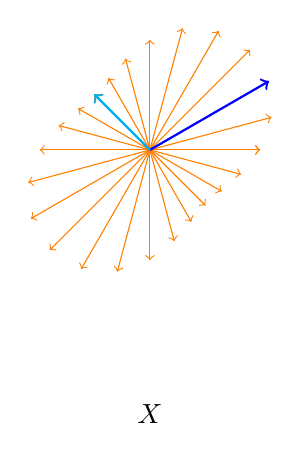
\begin{tikzpicture}
  \foreach \i [evaluate={\ang=\i*360/24;}] in {0,...,24}{
    \draw[->,orange] (\ang:0) --++ (\ang:{1.4+0.4*sin(2*\ang)});
  }
  \draw[->,thick,blue] (30:0) --++ (30:{1.4+0.4*sin(2*30)});
  \draw[->,thick,cyan] (135:0) --++ (135:{1.4+0.4*sin(2*135)});
  \node at (0,-2.4*1.4) {$X$};
\end{tikzpicture}&
$\xrightarrow[]{\mathbf{A}}$&
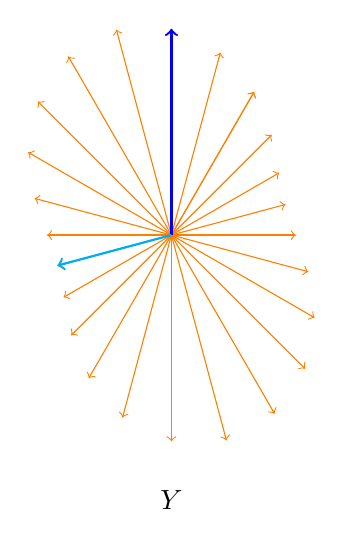
\begin{tikzpicture}
  \foreach \i [evaluate={\ang=\i*360/24;}] in {0,...,24}{
    \draw[->,orange] ({\ang+60}:0) --++ ({\ang+60}:{2.1+0.6*sin(2*\ang)});
  }
  \draw[->,thick,blue] ({30+60}:0) --++ ({30+60}:{2.1+0.6*sin(2*30)});
  \draw[->,thick, cyan] ({135+60}:0) --++ ({135+60}:{2.1+0.6*sin(2*135)});
  \node at (0,-2.4*1.4) {$Y$};
\end{tikzpicture}
\end{tabular}
\end{adjustbox}
\end{center}
\end{figure}
\end{exmp}

\clearpage

\section{Chapter II: Affine Spaces}
\subsection{Spaces}
\begin{defn}[Affine Space]\label{defafsp}
An affine space\index{affine space} with \hyperref[defrvs]{vector space} $T$ is a non-empty set $X$ and a difference function\index{difference function} $\mathbf{d}:X\times X \rightarrow T$\index{$\mathbf{d}$} such that for any $x,y,z \in X$
\begin{enumerate}
\item $\mathbf{d}(x,y)+\mathbf{d}(y,z)=\mathbf{d}(x,z)$
\item The restricted map\index{restricted map} $\mathbf{d}_x:\{x\}\times X \rightarrow T:(x,y)\mapsto \mathbf{d}(x,y)$\index{$\mathbf{d}_x$} is bijective
\end{enumerate}
The affine space is represented as $(X,T)$.
\end{defn}

\begin{cmnt*}That is, points are separated by vectors. Vectors go from one point to another in the affine space. Any two points are separated by vectors but it is not necessary from definition that given a starting point and a vector, there is an ending point such that the vector goes from the starting point to the ending point.\end{cmnt*}
\begin{cmnt*}The bijective condition allows us to define $x+\mathbf{t}$ for $x\in X$, $\mathbf{t}\in T$ as $y\in X$ such that $\mathbf{d}_x(x,y)=\mathbf{t}$.\end{cmnt*}
\begin{cmnt*}The first argument in the definition of $\mathbf{d}_x(x,y)$ is redundant. It is kept to indicate that $\mathbf{d}_x(x,y)$ operates on vectors starting at $x$ and ending at points in the affine space rather than directly on points in the affine space. An alternative notation could have been $\mathbf{d}_x((x,y))$ with the understanding that $(x,y)$ is a vector from $x$ to $y$.\end{cmnt*}

\begin{defn}[Tangent Space]\label{deftsp}
Given an \hyperref[defafsp]{affine space} $X$ with a difference function $\mathbf{d}$ and $x \in X$, the tangent space\index{tangent space} to $X$ at $x$, denoted $T_xX$\index{$T_x$} is the vector space $\{x\}\times X$ with the operations
\begin{enumerate}
\item $(x,y) + (x,z) = \mathbf{d}_x^{\leftarrow}\left( \mathbf{d}_x(x,y)+\mathbf{d}_x(x,z) \right)$
\item $(x,y)a = \mathbf{d}_x^{\leftarrow}\left( (\mathbf{d}_x(x,y))a \right)$
\end{enumerate}
\end{defn}

\begin{cmnt*}A tangent space to $X$ at $x$ consists of differences of all points of $X$ from $x$. These differences, called tangents\index{tangent}, are vectors from the definition of an affine space. Thus, tangents in a tangent space are vectors, except that they all start from the same point. That is, tangents are \textbf{bound vectors}\index{bound vector} but elements of the vector space underlying the affine space are \textbf{free vectors}\index{free vector}.\end{cmnt*}
\begin{cmnt*}The \hyperref[defafsp]{restricted difference function} $\mathbf{d}_x$ is called a freeing map\index{freeing map}. Its inverse $\mathbf{d}_x^{\leftarrow}$ that gives corresponding bound vector starting at $x$ is called a binding map\index{binding map}. A \hyperref[defafsp]{distance function} returns free vectors.\end{cmnt*}

\begin{exmp}
The red vectors are part of $T_xX$ and the blue vectors are part of $T_yX$.
\begin{figure}[H]
\begin{center}
\begin{adjustbox}{max totalsize={.7\textwidth}{.4\textheight},center}
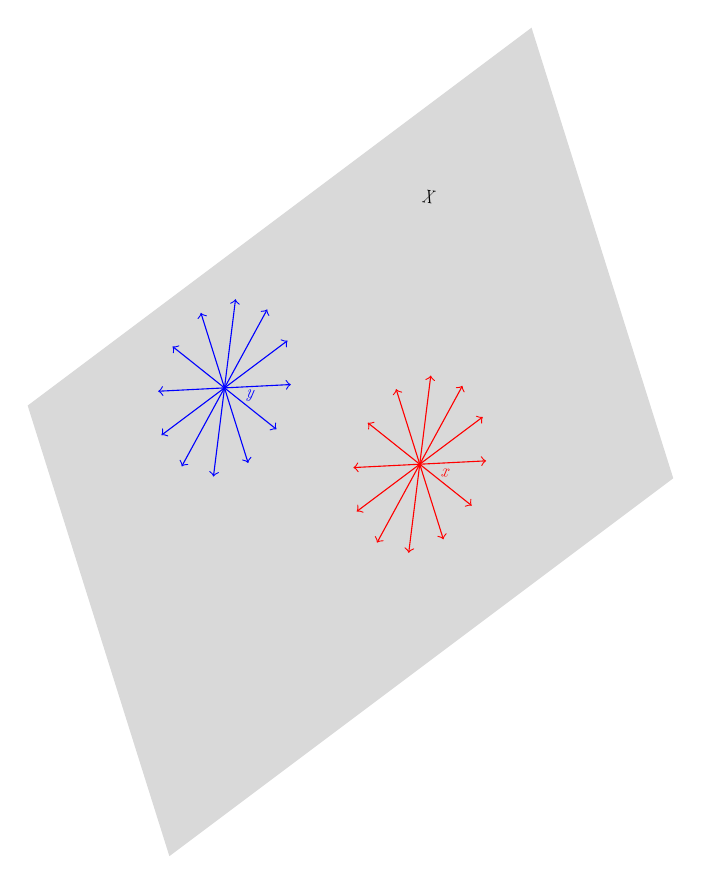
\begin{tikzpicture}[
    ->,
    plane x={(0.3,-0.9539)},
    plane y={(0.8,0.6)},
    canvas is plane,
]
    \fill[gray,fill opacity=0.3] (-3,-4) rectangle (3,4);
    \node at (1.1,1.1) [rotate=52,scale=0.6,transform shape,red] {$x$};
    \node at (-1.3,-1.1) [rotate=52,scale=0.6,transform shape,blue] {$y$};
    \node at (-2,2) [rotate=52,scale=0.6,transform shape] {$X$};
    \foreach \th in {0,30,...,330}
    {      
      \draw[red] (0.8,0.8) -- ({0.8+cos(\th)},{0.8+sin(\th)});
      \draw[blue] (-1.6,-1.4) -- ({-1.6+cos(\th)},{-1.4+sin(\th)});
    }
\end{tikzpicture}
\end{adjustbox}
\end{center}
\end{figure}
\end{exmp}

\begin{defn}[Dimension of Affine Space]
The dimension of an affine space\index{dimension of affine space} is the dimension of the space of its free vectors.
\end{defn}
\begin{exmp} All points on this page form an affine space of dimension two.
\end{exmp}

\begin{defn}[Weighted Average of Points in Affine Space]\label{defwaas}
Given affine space $(X,T)$, for $x,y\in X$, $(1-\lambda)x+\lambda y$ is defined as $x+\lambda\mathbf{d}(x,y)$.
\end{defn}
\begin{cmnt*}The above definition is generalized in obvious way to a weighted average of multiple points in an affine space.\end{cmnt*}
\begin{exmp} For the affine space of all points on this page, one-fourth of top-left corner and three-fourth of bottom right-corner is a point one-fourth distance along the diagonal from bottom right corner to top-left corner.
\end{exmp}

\subsection{Maps}
\begin{defn}[Affine Map]\label{defafmap}
If $X$ and $Y$ are \hyperref[defafsp]{affine spaces} with corresponding \hyperref[defrvs]{vector spaces} $T$ and $S$, respectively, a map $A:(X,T) \rightarrow (Y,S)$ is affine\index{affine map} if for any $x,x'\in X,\lambda \in \mathbb{R}$,
$$A((1-\lambda)x+\lambda x') = (1-\lambda)A(x) + \lambda Ax'.$$
\end{defn}

\begin{res} An affine map $A:(X,T) \rightarrow (Y,S)$ induces a \hyperref[deflinfvs]{linear map}, called the linear part of $A$, $\mathbf{A}:T\rightarrow S$\index{linear part of affine map} such that points separated by $\mathbf{t}\in T$ in $X$ are mapped to points separated by $\mathbf{At}\in S$ in $Y$.\end{res}
\begin{proof}
$\mathbf{A}$ is well-defined: Suppose $x,y,x',y'\in X$ such that $\mathbf{d}(x,y)=\mathbf{d}(x',y')$. Then,
\begin{align*}
&\frac{1}{2}x+\frac{1}{2}y'=x+\frac{1}{2}\mathbf{d}(x,y')=x+\frac{1}{2}(\mathbf{d}(x,y)+\mathbf{d}(y,x')+\mathbf{d}(x',y'))\\
&=x+\frac{1}{2}(\mathbf{d}(x,y)+2\mathbf{d}(y,x')+\mathbf{d}(x',y)+\mathbf{d}(x,y))\\
&=x+\mathbf{d}(x,y)+\mathbf{d}(y,x')+\frac{1}{2}\mathbf{d}(x',y)=x'+\frac{1}{2}\mathbf{d}(x',y)=\frac{1}{2}x'+\frac{1}{2}y.
\end{align*}
Then, by \autoref{defafmap}, $\frac{1}{2}A(x)+\frac{1}{2}A(y')=\frac{1}{2}A(x')+\frac{1}{2}A(y)$. That is, $A(x)+\frac{1}{2}\mathbf{d}(A(x),A(y'))=A(x')+\frac{1}{2}\mathbf{d}(A(x'),A(y))$. Substituting
\begin{align*}
&\mathbf{d}(A(x),A(y'))=\\
&\mathbf{d}(A(x),A(y))+\mathbf{d}(A(y),A(x'))+\mathbf{d}(A(x'),A(y'))=\\
&2\mathbf{d}(A(x),A(y))+2\mathbf{d}(A(y),A(x'))+\mathbf{d}(A(x'),A(y))+\mathbf{d}(A(x'),A(y'))-\mathbf{d}(A(x),A(y)),
\end{align*}
we get
\begin{align*}
&\frac{1}{2}A(x')+\frac{1}{2}\mathbf{d}(A(x'),A(y))+\frac{1}{2}(\mathbf{d}(A(x'),A(y'))-\mathbf{d}(A(x),A(y)))\\
&=\frac{1}{2}A(x')+\frac{1}{2}\mathbf{d}(A(x'),A(y))\\
&\implies \mathbf{d}(A(x'),A(y'))=\mathbf{d}(A(x),A(y)).
\end{align*}
$\mathbf{A}$ is a \hyperref[deflinfvs]{linear map}: Let $x,y,z\in X$ such that $\mathbf{d}(x,y)=\mathbf{s},\mathbf{d}(y,z)=\mathbf{t}$ and $\lambda\in\mathbb{R}$. Then, $\mathbf{A}(\mathbf{s})+\mathbf{A}(\mathbf{t}) = \mathbf{d}(A(x),A(y))+\mathbf{d}(A(y),A(z)) = \mathbf{d}(A(x),A(z))$ (by \autoref{defafsp} ) $= \mathbf{A}(\mathbf{s+t})$.

\noindent And $\mathbf{A}(\lambda\mathbf{s}) = \mathbf{d}(A(x),A(x+\lambda\mathbf{d}(x,y)))=\mathbf{d}(A(x),A((1-\lambda)x+\lambda y))$ (by \autoref{defwaas}) $=\mathbf{d}(A(x),(1-\lambda)A(x)+\lambda A(y))$ (by \autoref{defafmap}) $=\mathbf{d}(A(x),A(x)+\lambda\mathbf{d}(A(x),A(y)))$ (by \autoref{defwaas}) $=\lambda\mathbf{d}(A(x),A(y))=\lambda\mathbf{A}(\mathbf{s})$.
\end{proof}
\begin{exmp}
Take a picture of this page with a phone, possible slanted at an angle. The mapping from a point in the page to the corresponding point on the picture is an affine map.
\end{exmp}

\begin{defn}[Affine Isomorphism]
Given affine spaces $(X,T)$ and $(Y,S)$, an \hyperref[defafmap]{affine map} $A:X \rightarrow Y$ is an affine isomorphism\index{affine isomorphism} if there is an affine map $B:Y \rightarrow X$ such that $AB$ and $BA$ are identity maps.
\end{defn}

\begin{exmp}
Shadows from a distant light source such as sun of objects in a two-dimensional plane on another two-dimensional plane form an affine isomorphism. Shadows of objects in a three-dimensional space on a two-dimensional plane do not.
\end{exmp}

\begin{defn}[Affine Automorphism]
Given affine space $(X,T)$, an affine isomorphism $X \rightarrow X$ is an affine automorphism\index{affine automorphism}.
\end{defn}
\clearpage

\section{Chapter III: Dual Spaces}
\begin{defn}[Covariant and Contravariant Vectors]\label{defcoco}
Given a \hyperref[defrvs]{vector space} $X$, vectors in $X$ are called contravariant vectors\index{contravariant vector}. A \hyperref[deflinfvs]{linear map} from $X$ to $\mathbb{R}$ is called a covariant vector\index{covariant vector} or a dual vector\index{dual vector} or a linear functional\index{linear functional}.
\end{defn}

\begin{defn}[Dual Space] The space of linear functionals (\hyperref[defcoco]{covariant vectors}) on a vector space $X$ is denoted $L(X,\mathbb{R})$ or $X^*$\index{$X^*$}, and is called the dual space\index{dual space} of $X$.
\end{defn}

\begin{res} If $X$ is a vector space, then $X^*$ is a vector space.
\end{res}
\begin{proof}
Define addition and scalar multiplication in $X^*$ as pointwise addition of linear functionals and pointwise scalar multiplication. The result is also a \hyperref[defcoco]{linear functional}. $X^*$ satisfies \autoref{defrvs} of a vector space.
\end{proof}

\begin{exmp} If $X$ is the space of vectors in a 2-dimensional $x$-$y$ plane, the $x$-component of the vector, the $y$-component of the vector, the length of the vector, the cosine of the angle between the vector and the $x$-axis are all elements of $X^*$.
\end{exmp}

\begin{defn}[Dual Map]\label{defDMap} Given vector spaces $X$ and $Y$, and a \hyperref[deflinfvs]{linear map} $\mathbf{A}:X\rightarrow Y$, $\mathbf{A}^*$, the dual map\index{dual map} to $\mathbf{A}$ is $\mathbf{A}^*:Y^*\rightarrow X^*:\mathbf{f}\mapsto \mathbf{f}\circ \mathbf{A}$.
\end{defn}

\begin{cmnt*} If $\mathbf{A}:X\rightarrow Y$ is a linear map and $\mathbf{f}:Y\rightarrow\mathbb{R}$ is a linear functional on $Y$, then $\mathbf{g}=\mathbf{A}^*(\mathbf{f}):X\rightarrow\mathbb{R}$ is a linear functional on $X$ such that for all $\mathbf{x}\in X$, $\mathbf{g}(\mathbf{x})=\mathbf{f}(\mathbf{A}(\mathbf{x}))$.
\end{cmnt*}

\begin{exmp}
This is a continuation of Example \ref{exmplinfvs}.Both $X$ and $Y$ consist of vectors in two-dimensional plane. Map $\mathbf{A}$ scales a vector in $X$ by 1.5 and rotates it counterclockwise by $60^\circ$ to get its image in $Y$. Then, $\mathbf{A}^*$ maps any rule (same as linear functional) that assigns a number for each vector in $Y$ to a rule that assigns to each vector in $X$, the number for its corresponding vector in $Y$. For example, if the rule in $Y$ returns the polar angle (azimuth) of a vector, $\mathbf{A}^*$ maps this to a rule which returns the polar angle of a vector in $X$ plus $60^\circ$. If the rule in $Y$ returns the length of a vector, $\mathbf{A}^*$ maps this to a rule which returns 1,5 times the length of a vector in $X$.

\begin{figure}[H]
\begin{center}
\begin{adjustbox}{max totalsize={.9\textwidth}{.9\textheight},center}
\begin{tabular}{lcr}
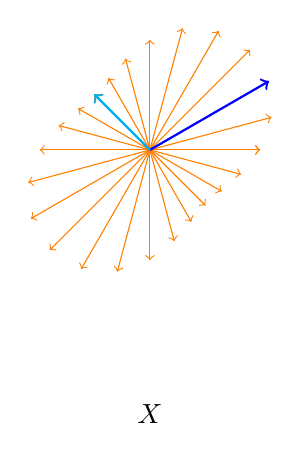
\begin{tikzpicture}
  \foreach \i [evaluate={\ang=\i*360/24;}] in {0,...,24}{
    \draw[->,orange] (\ang:0) --++ (\ang:{1.4+0.4*sin(2*\ang)});
  }
  \draw[->,thick,blue] (30:0) --++ (30:{1.4+0.4*sin(2*30)});
  \draw[->,thick,cyan] (135:0) --++ (135:{1.4+0.4*sin(2*135)});
  \node at (0,-2.4*1.4) {$X$};
\end{tikzpicture}&
$\xrightarrow[]{\mathbf{A}}$&
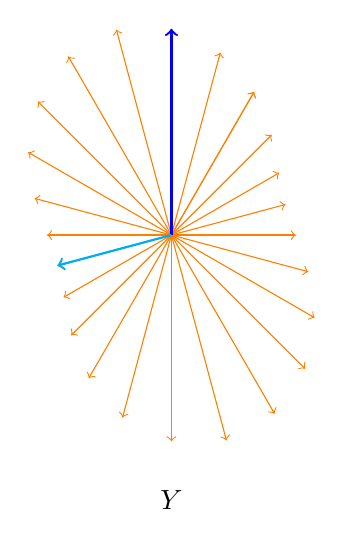
\begin{tikzpicture}
  \foreach \i [evaluate={\ang=\i*360/24;}] in {0,...,24}{
    \draw[->,orange] ({\ang+60}:0) --++ ({\ang+60}:{2.1+0.6*sin(2*\ang)});
  }
  \draw[->,thick,blue] ({30+60}:0) --++ ({30+60}:{2.1+0.6*sin(2*30)});
  \draw[->,thick, cyan] ({135+60}:0) --++ ({135+60}:{2.1+0.6*sin(2*135)});
  \node at (0,-2.4*1.4) {$Y$};
\end{tikzpicture}
\end{tabular}
\end{adjustbox}
\end{center}
\end{figure}
\end{exmp}

\begin{res} dim($X^*$)=dim($X$).\label{resdim}
\end{res}
\begin{proof}
Choose a basis\index{basis}\index{$\mathbf{b}_i$} $\beta=\mathbf{b}_1,\cdots,\mathbf{b}_n$ for $X$. Define $n$ linear functionals
\begin{align*}
\mathbf{b}^i:X\rightarrow \mathbb{R}:(a^1,\cdots,a^n)\mapsto a^i \textbf{ for }i=1,\cdots,n.
\end{align*}
\index{$\mathbf{b}^i$}Consider a linear functional $\mathbf{f}\in X^*$. For any $\mathbf{x}=(x^1,\cdots,x^n)\in X$,
\begin{align*}
\mathbf{f}(\mathbf{x})=\mathbf{f}(\sum_{i=1}^n x^i \mathbf{b}_i)=\sum_{i=1}^n x^i \mathbf{f}(\mathbf{b}_i)=\sum_{i=1}^n \mathbf{f}(\mathbf{b}_i) \mathbf{b}^i(\mathbf{x}).
\end{align*}
Thus, $\mathbf{f}=\sum_{i=1}^n \mathbf{f}(\mathbf{b}_i) \mathbf{b}^i$. That is, linear hull of $\mathbf{b}^1,\cdots,\mathbf{b}^n$ is $X^*$ (or $\mathbf{b}^1,\cdots,\mathbf{b}^n$ span $X^*$). Further, $\mathbf{b}^1,\cdots,\mathbf{b}^n$ are linearly independent because $\sum_{i=1}^n \alpha_i \mathbf{b}^i(\mathbf{x})=\sum_{i=1}^n \alpha_i x^i=0$ for all $\mathbf{x}$ only if $\alpha_1=\cdots=\alpha_n=0$. Thus, $\mathbf{b}^1,\cdots,\mathbf{b}^n$ is a basis of $X^*$.
\end{proof}
\begin{defn}[Dual Basis]\label{defdbas}
Given basis $\mathbf{b}_1,\cdots,\mathbf{b}_n$ of a vector space $X$, the basis of $X^*$, $\mathbf{b}^1,\cdots,\mathbf{b}^n$, defined in the proof above, is the dual basis\index{dual basis}.
\end{defn}

\begin{exmp}
For the two-dimensional vector space in $x$-$y$ plane, if the basis consists of unit vectors in $x$ and $y$ directions, then the dual basis consists of the $x$-coordinate and the $y$-coordinate.
\end{exmp}

\clearpage

\section{Chapter IV: Metric Vector Spaces}
\begin{defn}[Metric Tensor]\label{defmettns}
A metric tensor\index{metric tensor} on a vector space $X$ is a function $\mathbf{F}:X\times X\rightarrow \mathbb{R}$ which satisfies
\begin{enumerate}
\item $\mathbf{F}(\mathbf{x}+\mathbf{x}',\mathbf{y})=\mathbf{F}(\mathbf{x},\mathbf{y})+\mathbf{F}(\mathbf{x}',\mathbf{y})$
\item $\mathbf{F}(\mathbf{x},\mathbf{y}+\mathbf{y}')=\mathbf{F}(\mathbf{x},\mathbf{y})+\mathbf{F}(\mathbf{x},\mathbf{y}')$
\item $\mathbf{F}(\mathbf{x}a,\mathbf{y})=a\mathbf{F}(\mathbf{x},\mathbf{y})=\mathbf{F}(\mathbf{x},\mathbf{y}a)$
\item $\mathbf{F}(\mathbf{x},\mathbf{y})=\mathbf{F}(\mathbf{y},\mathbf{x})$ for all $\mathbf{x},\mathbf{y}\in X$
\item $\mathbf{F}(\mathbf{x},\mathbf{y})=0$ for all $\mathbf{y}\in X$ implies $\mathbf{x}=\mathbf{0}$
\end{enumerate}
\end{defn}

\begin{defn}[Inner Product]\label{definnpdt}
An inner product\index{inner product} on a vector space $X$ is a metric tensor on $X$ which is
\begin{enumerate}
\item positive definite\index{positive definite} $\mathbf{F}(\mathbf{x},\mathbf{x})>0$ for all $\mathbf{x}\neq \mathbf{0}$ or
\item negative definite\index{negative definite} $\mathbf{F}(\mathbf{x},\mathbf{x})<0$ for all $\mathbf{x}\neq \mathbf{0}$
\end{enumerate}
\end{defn}

\begin{defn}[Metric Vector Space]\label{defmetvs}
A metric vector space\index{metric vector space} $(X,\mathbf{G})$ is a vector space $X$ with a metric tensor $\mathbf{G}:X\times X \rightarrow \mathbb{R}$\index{$\mathbf{G}$}. We abbreviate $\mathbf{G}(\mathbf{x},\mathbf{y})$ to $\mathbf{x}\cdot\mathbf{y}$\index{$\mathbf{x}\cdot\mathbf{y}$}.
\end{defn}

\begin{defn}[Inner Product Space]\label{definpsp}
An inner product space\index{inner product space} $(X,\mathbf{G})$ is a vector space $X$ with an inner product $\mathbf{G}:X\times X \rightarrow \mathbb{R}$.
\end{defn}

\begin{defn}[Standard Inner Product on $\mathbb{R}^n$]\label{defsip}
The standard inner product\index{standard inner product} on $\mathbb{R}^n$ is defined by
\begin{align*}
(x^1,\cdots,x^n)\cdot(y^1,\cdots,y^n)=\sum_{i=1}^n x^iy^i.
\end{align*}
\end{defn}

\begin{defn}[Lorentz Metric on $\mathbb{R}^4$]\label{defLmet}
The Lorentz metric\index{Lorentz metric} on $\mathbb{R}^4$ is defined by
\begin{align*}
(x^0,x^1,x^2,x^3)\cdot(y^0,y^1,y^2,y^3)= x^0y^0 - x^1y^1 - x^2y^2 - x^3y^3.
\end{align*}
\end{defn}

\begin{cmnt*}
The \hyperref[defsip]{standard inner product} is an \hyperref[definnpdt]{inner product}. Lorentz metric is a \hyperref[defmettns]{metric tensor}, but not an \hyperref[definnpdt]{inner product}.
\end{cmnt*}

\begin{defn}[Length]\label{deflen}
In a metric vector space $(X,\mathbf{G})$, the length\index{length} of $\mathbf{x}\in X$ is $|x|_{\mathbf{G}}=\sqrt{\mathbf{x}\cdot\mathbf{x}}$\index{$\vert x\vert_{\mathbf{G}}$}.
\end{defn}

\begin{cmnt*}
The \hyperref[deflen]{length} may be real or imaginary. Nonzero lengths are always real or always imaginary in an \hyperref[definpsp]{inner product space}.
\end{cmnt*}

\begin{defn}[Norm]\label{defnorm}
A norm\index{norm} on a vector space $X$ is a function $X\rightarrow \mathbb{R}: \mathbf{x} \mapsto ||\mathbf{x}||$\index{$\Vert \mathbf{x}\Vert$} such that for all $\mathbf{x},\mathbf{y} \in X$ and $a \in \mathbb{R}$,
\begin{enumerate}
\item $||\mathbf{x}||=0$ implies $\mathbf{x}=\mathbf{0}$,
\item $||\mathbf{x}a||=|a|\,||\mathbf{x}||$, and
\item $||\mathbf{x+y}|| \le ||\mathbf{x}|| + ||\mathbf{y}||$.
\end{enumerate}
\end{defn}

\begin{defn}[Partial Norm]\label{defpnorm}
A partial norm\index{partial norm} on a vector space $X$ is a function $X\rightarrow \mathbb{R}: \mathbf{x} \mapsto ||\mathbf{x}||$ such that for all $\mathbf{x},\mathbf{y} \in X$ and $a \in \mathbb{R}$,
\begin{enumerate}
\item $||\mathbf{x}|| \ge 0$ for all $\mathbf{x} \in X$ and
\item $||\mathbf{x}a||=|a|\,||\mathbf{x}||$.
\end{enumerate}
\end{defn}

\begin{cmnt*}
A \hyperref[defmettns]{metric tensor} assigns a number to a pair of vectors, while a \hyperref[defnorm]{norm} assigns a number to each vector.
\end{cmnt*}

\begin{exmp}
In the space of vectors in $x$-$y$ plane, the absolute value of $x$ component is a partial norm, but not a norm.  
\end{exmp}

\begin{defn}\label{defsize}
A metric tensor $\mathbf{G}$ can be used to get a norm: $||\mathbf{x}|| \equiv ||\mathbf{x}||_\mathbf{G} = \sqrt{|\mathbf{G}(\mathbf{x},\mathbf{x})|}$, called the size\index{size} of $\mathbf{x}$. The size is the same as the \hyperref[deflen]{length} $|\mathbf{x}|_\mathbf{G}$ if $\mathbf{G}$ is an \hyperref[definnpdt]{inner product}.
\end{defn}

\begin{defn}\label{defunit}
A unit vector\index{unit vector} $\mathbf{x}\in X$ in a metric vector space $(X,\mathbf{G})$ is a vector of \hyperref[defsize]{size} 1: $||\mathbf{x}||_\mathbf{G}=1$.
\end{defn}

\begin{res}In an inner product space $(X,\mathbf{G})$, for any $\mathbf{x},\mathbf{y} \in X$, we have $\mathbf{x}\cdot\mathbf{y} \le |\mathbf{x}|\,|\mathbf{y}|$ with equality for non-zero $\mathbf{x},\mathbf{y}$ only if $\mathbf{y}=\mathbf{x}a$ for $a \in \mathbb{R}$.
\end{res}
\begin{proof}
For any $a\in \mathbb{R}$,
\begin{align*}
(\mathbf{x}a-\mathbf{y})\cdot(\mathbf{x}a-\mathbf{y}) = (\mathbf{x}\cdot\mathbf{x})a^2 - (2\mathbf{x}\cdot\mathbf{y}) + \mathbf{y}\cdot\mathbf{y} \ge 0.
\end{align*}
This requires that the discriminant of the quadratic in $a$ be non-positive:
\begin{align*}
&(2\mathbf{x}\cdot\mathbf{y})^2 - 4(\mathbf{x}\cdot\mathbf{x})(\mathbf{y}\cdot\mathbf{y}) \le 0\\
&\implies \mathbf{x}\cdot\mathbf{y} \le |\mathbf{x}|\,|\mathbf{y}|.
\end{align*}
With equality, there is a single value of $a$ for which $\mathbf{x}a-\mathbf{y} = \mathbf{0}$.
\end{proof}

\begin{defn}[Orthogonal Vectors]\label{defortho}
Two vectors $\mathbf{x}$,$\mathbf{y}$ in a metric vector space are orthogonal\index{orthogonal vectors} if $\mathbf{x}\cdot\mathbf{y}=0$.
\end{defn}
\clearpage

\section{Chapter V: Tensors and Multilinear Forms}
\begin{defn}[Multilinear Mapping]\label{defmmap}
A function $\mathbf{f}:X_1 \times X_2 \times \cdots X_n \rightarrow Y$ where $X_1,\cdots,X_n,Y$ are vector spaces, is a multilinear mapping\index{multilinear mapping} if
\begin{enumerate}
\item $\mathbf{f}(\mathbf{x}_1,\cdots,\mathbf{x}_i+\mathbf{x}_i',\cdots,\mathbf{x}_n) = \mathbf{f}(\mathbf{x}_1,\cdots,\mathbf{x}_i,\cdots,\mathbf{x}_n) + \mathbf{f}(\mathbf{x}_1,\cdots,\mathbf{x}_i,\cdots,\mathbf{x}_n)$
\item $\mathbf{f}(\mathbf{x}_1,\cdots,\mathbf{x}_ia,\cdots,\mathbf{x}_n) = \left( \mathbf{f}(\mathbf{x}_1,\cdots,\mathbf{x}_i,\cdots,\mathbf{x}_n) \right)a$
\end{enumerate}
for any $x_1\in X_1, \cdots, x_n\in X_n$, and $x_1'\in X_1, \cdots, x_n'\in X_n$, $i\in \{1,\cdots,n\}$, and $a\in \mathbb{R}$. The vector space of all such functions is denoted by $L(X_1,\cdots,X_n;Y)$\index{$L(X_1,\cdots,X_n;Y)$}.
\end{defn}
\begin{defn}[Multilinear Form]\label{defmform}
A multilinear form\index{multilinear form} on $\mathbf{X}$ is a multilinear mapping $\mathbf{f}\in L^n(X;Y) \equiv L(\overbrace{X,\cdots,X}^{n \text{ times}};Y)$\index{$L^n(X;Y)$}.
\end{defn}
\begin{exmp} If $\mathbf{X}$ is a three-dimensional space, then $\mathbf{f}(\mathbf{x}_1,\mathbf{x}_2,\mathbf{x}_3)$, the signed volume (following left-hand rule) of a parallelopiped formed by $\mathbf{x}_1,\mathbf{x}_2,\mathbf{x}_3\in\mathbf{X}$ is a multilinear form..
\end{exmp}

\begin{defn}[Tensor Product of Spaces]\label{deftprod}
A tensor product\index{tensor product of spaces} of vector spaces $\mathbf{X}_1,\cdots,\mathbf{X}_n$ is a space $\mathbf{X}$ together with a map\index{$\bigotimes$}
\begin{align*}
\bigotimes:\mathbf{X}_1 \times \mathbf{X}_2 \times \cdots \times \mathbf{X}_n \rightarrow \mathbf{X}
\end{align*}
such that
\begin{enumerate}
\item $\bigotimes:\mathbf{X}_1 \times \mathbf{X}_2 \times \cdots \times \mathbf{X}_n \rightarrow \mathbf{X}$ is multilinear
\item If $\mathbf{f}:\mathbf{X}_1 \times \mathbf{X}_2 \times \cdots \times \mathbf{X}_n \rightarrow \mathbf{Y}$ is multilinear, then there is a unique linear map
\begin{align*}
\hat{\mathbf{f}}:\mathbf{X} \rightarrow \mathbf{Y}
\end{align*}
such that $\mathbf{f} = \hat{\mathbf{f}} \circ \bigotimes$.
\end{enumerate}
\end{defn}

\begin{cmnt*}
The tensor product space in \autoref{deftprod} needs to have addition operation for linearity to make sense. However, it is not necessarily closed under addition so it is not necessarily a vector space. To create a vector space, linear combinations of image of $\bigotimes$ should be included in the space.
\end{cmnt*}

\begin{exmp} \label{exmpTP} If $\mathbf{X}_1^*, \mathbf{X}_2^*, \cdots \mathbf{X}_n^*$ are dual spaces for vector spaces $\mathbf{X}_1, \mathbf{X}_2, \cdots \mathbf{X}_n$, respectively, the following mapping is a tensor product of spaces $\mathbf{X}_1^*, \mathbf{X}_2^*, \cdots \mathbf{X}_n^*$
\begin{align*}
\bigotimes:\mathbf{X}_1^* \times \mathbf{X}_2^* \times \cdots \times \mathbf{X}_n^* &\rightarrow L(\mathbf{X}_1,\cdots,\mathbf{X}_n;\mathbb{R}): \\
(\mathbf{g}_1,\mathbf{g}_2,\cdots,\mathbf{g}_n) &\mapsto \mathbf{g}_1 \otimes \mathbf{g}_2 \otimes \cdots \otimes \mathbf{g}_n 
\end{align*}
where $\mathbf{g}_1 \otimes \mathbf{g}_2 \otimes \cdots \otimes \mathbf{g}_n$ is the \hyperref[defmmap]{multilinear mapping}
\begin{align*}
\mathbf{g}_1 \otimes \mathbf{g}_2 \otimes \cdots \otimes \mathbf{g}_n: \mathbf{X}_1 \times  \mathbf{X}_2 \times \cdots \times \mathbf{X}_n &\rightarrow \mathbb{R}: \\
(\mathbf{x}_1,\mathbf{x}_2,\cdots,\mathbf{x}_n) &\mapsto \mathbf{g}_1(\mathbf{x}_1)\mathbf{g}_2(\mathbf{x}_2)\cdots \mathbf{g}_n(\mathbf{x}_n).
\end{align*}
Requirement 1 in the \hyperref[deftprod]{definition} of tensor product is clearly satisfied. For requirement 2, let $\mathbf{b}_{i1},\mathbf{b}_{i2},\cdots,\mathbf{b}_{ik_i}$ be a basis for $\mathbf{X}_i$ and let $\mathbf{b}_i^1,\mathbf{b}_i^2,\cdots,\mathbf{b}_i^{k_i}$ be the corresponding \hyperref[defdbas]{dual basis}\index{dual basis} for $\mathbf{X}_i^*$. Then, for $\mathbf{h}\in L(\mathbf{X}_1,\cdots,\mathbf{X}_n;\mathbb{R})$, $\mathbf{x}_1 \in \mathbf{X}_1,\mathbf{x}_2 \in \mathbf{X}_2,\cdots,\mathbf{x}_n \in \mathbf{X}_n$,
\begin{align*}
&\mathbf{h}(\mathbf{x}_1,\mathbf{x}_2,\cdots,\mathbf{x}_n) = \mathbf{h}\left(\sum_{j_1=1}^{k_1}a_1^{j_1} \mathbf{b}_{1j_1},\sum_{j_2=1}^{k_2}a_2^{j_2} \mathbf{b}_{2j_2},\cdots,\sum_{j_n=1}^{k_n}a_n^{j_n} \mathbf{b}_{nj_n}\right) \\
&= \sum_{j_1=1}^{k_1}\sum_{j_2=1}^{k_2}\cdots \sum_{j_n=1}^{k_n} a_1^{j_1}a_2^{j_2}\cdots a_n^{j_n} \mathbf{h}(\mathbf{b}_{1j_1}, \mathbf{b}_{2j_2},\cdots, \mathbf{b}_{nj_n}) \\
&= a_1^{j_1}a_2^{j_2}\cdots a_n^{j_n} \mathbf{h}(\mathbf{b}_{1j_1}, \mathbf{b}_{2j_2},\cdots, \mathbf{b}_{nj_n})\\
&= \mathbf{h}(\mathbf{b}_{1j_1}, \mathbf{b}_{2j_2},\cdots, \mathbf{b}_{nj_n}) \mathbf{b}_1^{j_1}\otimes \mathbf{b}_2^{j_2}\otimes \cdots \otimes \mathbf{b}_n^{j_n}(\mathbf{x}_1,\mathbf{x}_2,\cdots,\mathbf{x}_n).
\end{align*}
Thus, $\mathbf{h}$ has a unique representation as $h_{j_1j_2\cdots j_n} \mathbf{b}_1^{j_1}\otimes \mathbf{b}_2^{j_2}\otimes \cdots \otimes \mathbf{b}_n^{j_n}$ where $h_{j_1j_2\cdots j_n} = \mathbf{h}(\mathbf{b}_{1j_1}, \mathbf{b}_{2j_2},\cdots, \mathbf{b}_{nj_n})$. Now, if $\mathbf{f}:\mathbf{X}_1^* \times \mathbf{X}_2^* \times \cdots \times \mathbf{X}_n^* \rightarrow \mathbf{Y}$ is multilinear, define $\hat{\mathbf{f}}: L(\mathbf{X}_1,\cdots,\mathbf{X}_n;\mathbb{R}) \rightarrow \mathbf{Y}$ as
\begin{align*}
\hat{\mathbf{f}}: h_{j_1j_2\cdots j_n} \mathbf{b}_1^{j_1}\otimes \mathbf{b}_2^{j_2}\otimes \cdots \otimes \mathbf{b}_n^{j_n} \mapsto  h_{j_1j_2\cdots j_n} \mathbf{f}\left(\mathbf{b}_1^{j_1},\mathbf{b}_2^{j_2}, \cdots, \mathbf{b}_n^{j_n} \right).
\end{align*}
The mapping is, by definition, linear. It satisfies $\mathbf{f}=\hat{\mathbf{f}}\circ \bigotimes$. It is unique because any other linear mapping should match $\hat{\mathbf{f}}$ on all $\mathbf{b}_1^{j_1}\otimes \mathbf{b}_2^{j_2}\otimes \cdots \otimes \mathbf{b}_n^{j_n}$ and, therefore, by linearity, match on all $L(\mathbf{X}_1,\cdots,\mathbf{X}_n;\mathbb{R})$. 
\end{exmp}

\begin{res} \label{resuniqtp} A tensor product of vector spaces $\mathbf{X}_1,\cdots,\mathbf{X}_n$ exists, and any two are isomorphic.
\end{res}
\begin{proof}
Existence follows from Example \ref{exmpTP} after replacing each $\mathbf{X}_i$ with $\mathbf{X}_i^*$. Suppose $\bigotimes:\mathbf{X}_1 \times \mathbf{X}_2 \times \cdots \times \mathbf{X}_n \rightarrow \mathbf{X}$ and $\bigotimes':\mathbf{X}_1 \times \mathbf{X}_2 \times \cdots \times \mathbf{X}_n \rightarrow \mathbf{X}'$ are both tensor products. Then, from the \hyperref[deftprod]{definition} of tensor product, there exist unique $\mathbf{\Psi}$ and $\mathbf{\Phi}$ such that $\bigotimes=\mathbf{\Psi}\bigotimes'$ and $\bigotimes'=\mathbf{\Phi}\bigotimes$. These imply $\mathbf{\Psi}\mathbf{\Phi}\bigotimes=\mathbf{I}_X\bigotimes$ and $\mathbf{\Phi}\mathbf{\Psi}\bigotimes'=\mathbf{I}_{X'}\bigotimes'$. Since $\mathbf{I}_X\bigotimes$ is multilinear, so is $\mathbf{\Psi}\mathbf{\Phi}\bigotimes$. Then, by the uniqueness property in part 2 of the \hyperref[deftprod]{definition} of tensor product, $\mathbf{I}_X=\mathbf{\Psi}\mathbf{\Phi}$. Similarly, $\mathbf{I}_{X'}=\mathbf{\Phi}\mathbf{\Psi}$. Thus, $\mathbf{X} \cong \mathbf{X}'.$
\end{proof}

\begin{defn}[Tensor Product and Tensor Product of Spaces]\label{defttprod}
The tensor product of vector spaces $\mathbf{X}_1,\cdots,\mathbf{X}_n$ defined in Definition \ref{deftprod} (unique upto an isomorphism from Result \ref{resuniqtp}) is represented as $\mathbf{X}_1 \otimes \cdots \otimes \mathbf{X}_n$\index{$\mathbf{X}_1 \otimes \cdots \otimes \mathbf{X}_n$}. For $\mathbf{x}_1\in X_1,\cdots,\mathbf{x}_n\in X_n$, the image of $(\mathbf{x}_1,\cdots,\mathbf{x}_n)$ under $\mathbf{X}_1 \otimes \cdots \otimes \mathbf{X}_n$ is called the tensor product\index{tensor product} of $\mathbf{x}_1,\cdots,\mathbf{x}_n$ and is denoted by $\mathbf{x}_1 \otimes \cdots \otimes \mathbf{x}_n$\index{$\mathbf{x}_1 \otimes \cdots \otimes \mathbf{x}_n$}.
\end{defn}

\begin{cmnt*} From \autoref{exmpTP} and \autoref{defttprod}, if $\mathbf{x}_1\in X_1,\cdots,\mathbf{x}_n\in X_n$, the tensor product $\mathbf{x}_1 \otimes \cdots \otimes \mathbf{x}_n \in L(X_1^*,\cdots,X_n^*;\mathbb{R})$ is a linear functional on $X_1^*\times\cdots\times X_n^*$.
\end{cmnt*}

\begin{res} \label{resmptensr} For any two vector spaces $\mathbf{X}_1$, $\mathbf{X}_2$, there is an isomorphism
\[ L(X_1;X_2) \rightarrow X_1^* \otimes X_2.\]
\end{res}
\begin{proof}
Define
\begin{align*}
\mathbf{f}:X_1^*\times X_2 &\rightarrow L(X_1;X_2)\\
(\mathbf{g},\mathbf{x}_2) &\mapsto \left( \mathbf{x}_1 \mapsto (\mathbf{x_2)(\mathbf{g}(\mathbf{x}_1))}\right).
\end{align*}
Since $\mathbf{f}$ is multilinear, by part 2 of the \hyperref[deftprod]{definition} of tensor product, there is a linear map
\[ \hat{\mathbf{f}}:X_1^* \otimes X_2 \rightarrow L(X_1,X_2) \text{ with }\hat{\mathbf{f}}\bigotimes = \mathbf{f}. \]
Then, $\hat{\mathbf{f}}(\mathbf{g}\otimes \mathbf{x}_2) = \mathbf{0} \implies  \mathbf{f}(\mathbf{g}, \mathbf{x}_2) = \mathbf{0} \implies  (\mathbf{x}_2)(\mathbf{g}(\mathbf{x}_1)) = \mathbf{0} \forall \mathbf{x}_1 \implies \mathbf{g}\otimes \mathbf{x}_2 = \mathbf{0}.$ This ensures that $\hat{\mathbf{f}}$ is injective (no two elements map to same image, we have only shown it for elements of the form $\mathbf{g}\otimes \mathbf{x}_2$, technically, we should show it for linear combinations of such terms too.). Finally, $dim(X_1^*\otimes X_2) = dim(X_1^*)dim(X_2) = dim(X_1)dim(X_2) = dim(L(X_1;X_2))$. Thus, $L(X_1;X_2)$ and $X_1^* \otimes X_2$ are isomorphic.
\end{proof}

\begin{cmnt*} \autoref{resmptensr} states that $X_1^* \otimes X_2$ and $L(X_1;X_2)$ are isomorphic. Previous comment states that $X_1^* \otimes X_2$ and $L(X_1,X_2^*;\mathbb{R})$ are isomorphic. These two are consistent because $L(X_1;X_2)$ and $L(X_1,X_2^*;\mathbb{R})$ are isomorphic. An element in $L(X_1;X_2)$ maps a vector in $X_1$ to an image vector in $X_2$. The corresponding element in $L(X_1,X_2^*;\mathbb{R})$ returns a real number by applying a functional in $\mathbf{X}_2^*$ to the image vector.
\end{cmnt*}

\begin{defn}[Tensors]\label{deftnsr}
Vectors in the tensor product space $X_h^k$\index{$X_h^k$} of the type
\begin{align*}
\underbrace{X \otimes X \otimes \cdots \otimes X}_{k \text{ times}} \otimes \underbrace{X^* \otimes X^* \otimes \cdots \otimes X^*}_{h \text{ times}}
\end{align*}
for some space $X$ are called tensors\index{tensor} on $X$, covariant\index{covariant} of degree $h$, contravariant\index{contravariant} of degree $k$, or of type $\binom{k}{h}$.
\end{defn}

\begin{cmnt*} When the definition says ``vectors in the tensor product space,'' it does not mean contravariant vectors in $X$ (or covariant vectors in $X^*$). A tensor covariant of degree $h$ and contravariant of degree $k$ can be thought of as a rule that linearly acts on $h$ contravariant vectors and $k$ covariant vectors to give a real number.
\end{cmnt*}

\begin{res} dim($X_h^k$)=dim$(X)^{h+k}$.\index{dimension of tensor}
\end{res}
\begin{proof}
Example \ref{exmpTP} shows that tensor products of the form $\mathbf{b}_1^{j_1}\otimes \mathbf{b}_2^{j_2}\otimes \cdots \otimes \mathbf{b}_n^{j_n}$ form a basis for $L(\mathbf{X}_1,\cdots,\mathbf{X}_n;\mathbb{R})$ so dim$(L(\mathbf{X}_1,\cdots,\mathbf{X}_n;\mathbb{R}))=k_1k_2\cdots k_n$. The result follows from Replacing $n$ with $h+k$, each of $\mathbf{X}_1,\cdots,\mathbf{X}_h$ with $\mathbf{X}$, each of $\mathbf{X}_{h+1},\cdots,\mathbf{X}_n$ with $\mathbf{X}^*$, and noting dim($\mathbf{X}^*$)=dim($\mathbf{X}$) (see Result \ref{resdim}).
\end{proof}

\begin{exmp} \leavevmode
\begin{itemize}
\item A scalar is a tensor of type $\binom{0}{0}$. It returns a number without any arguments.
\item A \hyperref[defcoco]{contravariant vector} is a tensor of type $\binom{1}{0}$. It can be applied to a covariant vector to get a number (for example, $x$-coordinate).
\item A \hyperref[defcoco]{covariant vector} (a linear functional) is a tensor of type $\binom{0}{1}$. It can be applied to a contravariant vector to get a number.
\item A \hyperref[defmettns]{metric tensor} is a tensor of type $\binom{0}{2}$. It is applied to two contravariant vectors to get a number. 
\item A \hyperref[deflinfvs]{linear mapping} $X\rightarrow X$ is a tensor of type $\binom{1}{1}$, as given a vector and a functional, the functional applied to the image of the linear mapping is a scalar that is linear in the vector and also linear in the functional. This is a special case of Result \ref{resmptensr}.
\item At a point in $\mathbb{R}^3$, for any unit vector $\mathbf{v}$, Cauchy stress tensor $\mathbf{T}(\mathbf{v})$ is a vector representing the stress (force per area) along the plane perpendicular to $\mathbf{v}$ at the point. Cauchy's postulate states that the stress is a function of the normal vector $\mathbf{v}$ only, and is not influenced by the curvature of the surface. Cauchy's stress theorem states that the stress is a linear function of $\mathbf{v}$. Since a linear combination of unit vectors is not necessarily a unit vector, we can generalize the definition to non-unit vectors as $\mathbf{T}(\mathbf{v})$ is $|v|$ times a vector representing the force per area, along the plane perpendicular to $\mathbf{\mathbf{v}}$. Then, Cauchy stress tensor is a linear mapping from vectors in $\mathbb{R}^3$ to vectors in $\mathbb{R}^3$, and is thus, isomorphic to a tensor of type $\binom{1}{1}$ on the space of vectors in $\mathbb{R}^3$.
\end{itemize}
\end{exmp}

\begin{defn}[Contraction]\label{defcontr}
Given a tensor product space
\begin{align*}
\underbrace{X \otimes X \otimes \cdots \otimes X}_{k \text{ times}} \otimes \underbrace{X^* \otimes X^* \otimes \cdots \otimes X^*}_{h \text{ times}},
\end{align*}
the \hyperref[deflinfvs]{linear mapping}
\begin{align*}
\underbrace{X \otimes X \otimes \cdots \otimes X}_{k \text{ times}} \otimes \underbrace{X^* \otimes X^* \otimes \cdots \otimes X^*}_{h \text{ times}} \rightarrow \underbrace{X \otimes X \otimes \cdots \otimes X}_{k-1 \text{ times}} \otimes \underbrace{X^* \otimes X^* \otimes \cdots \otimes X^*}_{h-1 \text{ times}}:\\
\mathbf{x}_1 \otimes \cdots \otimes \mathbf{x}_{i-1} \otimes \mathbf{x}_i \otimes \mathbf{x}_{i+1} \otimes \cdots \otimes \mathbf{x}_{k} \otimes \mathbf{f}^{1} \otimes \cdots \otimes \mathbf{f}^{j-1} \otimes \mathbf{f}^j \otimes \mathbf{f}^{j+1} \otimes \cdots \otimes \mathbf{f}^{h} \\
\mapsto \left(\mathbf{x}_1 \otimes \cdots \otimes \mathbf{x}_{i-1} \otimes \mathbf{x}_{i+1} \otimes \cdots \otimes \mathbf{x}_{k} \otimes \mathbf{f}^{1} \otimes \cdots \otimes \mathbf{f}^{j-1} \otimes \mathbf{f}^{j+1} \otimes \cdots \otimes \mathbf{f}^{h}\right) \mathbf{f}^j(\mathbf{x}_i)
\end{align*}
is called a contraction map\index{contraction map} and the image of a tensor $\mathbf{x}$ in $\mathbf{X}$ under this map is called a contraction\index{contraction} of $\mathbf{x}$.
\end{defn}
\clearpage

\section{Chapter VI: Topological Vector Spaces}
\subsection{Continuity}
\begin{defn}[Metric]\label{defmtrc}
A metric\index{metric} on a set $X$ is a function $d:X \times X \rightarrow \mathbb{R}$ satisfying
\begin{enumerate}
\item $d(x,y) = d(y,x)$
\item $d(x,y)=0$ if and only if $x=y$
\item $d(x,z)\le d(x,y)+d(y,z)$.
\end{enumerate}
The pair $(X,d)$\index{$(X,d)$} is called a metric space.
\end{defn}
\begin{defn}[Semimetric]\label{defsmtr}
A semimetric\index{semimetric} or pseudometric\index{pseudometric} on a set $X$ is a function $d:X \times X \rightarrow \mathbb{R}$ satisfying
\begin{enumerate}
\item $d(x,y) = d(y,x)$
\item $d(x,x)=0$
\item $d(x,z)\le d(x,y)+d(y,z)$.
\end{enumerate}
\end{defn}

\begin{defn}[Continuous Function]\label{defcont}
A function $f:X\rightarrow Y$ between metric spaces $(X,d)$ and $(Y,d')$ is continuous\index{continuous function between metric spaces} at $x\in X$ if for any $0<\epsilon\in \mathbb{R}$ there exists $0<\delta\in \mathbb{R}$ such that if $d(x,y)<\delta$ then $d'\left( f(x),f(y)\right)<\epsilon$. A function is continuous on $S\in X$ if it is continuous at all $x\in S$. A function is continuous if it is continuous at all $x\in X$.
\end{defn}

\begin{defn}[Open Ball]\label{defoball}
Given a metric space $(X,d)$, $x\in X$, and $0<\delta\in \mathbb{R}$, the set $\{y|d(x,y)<\delta\}$ is called the open ball\index{open ball} $B(x,\delta)$\index{$B(x,\delta)$} of radius $\delta$ around $x$.
\end{defn}

\begin{defn}[Boundary Point]\label{defbpnt}
A boundary point\index{boundary point} or point of closure\index{point of closure} of a set $S$ in a metric space $(X,d)$ is a point $x$ such that for any $0<\delta\in\mathbb{R}$, $B(x,\delta)$ contains both points in $S$ and points not in $S$.
\end{defn}

\begin{defn}[Open Set]\label{defoset}
A set in a metric space is open\index{open set} if it does not contain any boundary points it has.
\end{defn}

\begin{defn}[Closed Set]\label{defcset}
A set in a metric space is closed\index{closed set} if it contains all its boundary points.
\end{defn}

\begin{res} An open ball is an open set.\label{resoball}
\end{res}
\begin{proof}
Given a metric space $(X,d)$, and an open ball $B(x,\delta)$ with $x\in X$ and $0<\delta\in \mathbb{R}$, consider $x'\in B(x,\delta)$. Let $\epsilon=\left(\delta-d(x,x')\right)/2$. Clearly, $\epsilon>0$ and for any $y\in B(x',\epsilon)$, $d(x,y)\le d(y,x')+d(x',x)<\delta \implies y\in B(x,\delta)$. Thus, $x'$ is not a \hyperref[defbpnt]{boundary point} of $B(x,\delta)$.
\end{proof}

\begin{res}\label{rescontx}
A function $f:X\rightarrow Y$ between two metric spaces is continuous at $x\in X$ if and only if for any open set $V$ containing $f(x)$, there is an open set $U$ containing $x$ such that $f(U)\subseteq V$.
\end{res}
\begin{proof}
\textbf{Only If}: If $V$ is an \hyperref[defoset]{open set} containing $f(x)$, $f(x)$ is not a \hyperref[defbpnt]{boundary point} of $V$, so there exists $0<\epsilon\in \mathbb{R}$ such that $B(f(x),\epsilon)\subseteq V$. If $f$ is continuous at $x$, there exists $0<\delta\in \mathbb{R}$ such that $d(x,y)<\delta\implies d(f(x),f(y))<\epsilon$. Hence, $U=B(x,\delta)$ is an open set (see Result \ref{resoball}) containing $x$ and $f(U)\subseteq B(f(x),\epsilon)\subseteq V$.

\noindent \textbf{If}: Suppose for any open set $V$ containing $f(x)$, there is an open set $U$ containing $x$ such that $f(U)\subseteq V$. Given $0<\epsilon\in \mathbb{R}$, choose $V=B(f(x),\epsilon)$.  Then, there exists an open set $U$ containing $x$ such that $f(U)\subseteq B(f(x),\epsilon)$. By \hyperref[defoset]{definition} of open set, $x$ is not a \hyperref[defbpnt]{boundary point} of $U$, so there exists $0<\delta\in \mathbb{R}$ such that $B(x,\delta)\subseteq U$. Then, for any $x'\in X$ such that $d(x,x')<\delta$, $x'\in B(x,\delta) \subseteq U$ and therefore, $f(x)\in f(U)\subseteq B(f(x),\epsilon)\implies d(f(x),f(x'))<\epsilon$.
\end{proof}

\begin{res}\label{rescontf}
A map $f:X\rightarrow Y$ between two metric spaces is continuous if and only if $f^{\leftarrow}(V)$ is open for each open set $V$ in $Y$.
\end{res}
\begin{proof}
\textbf{Only If}: If $f$ is continuous and $V$ is an \hyperref[defoset]{open set} in $Y$, for each $x\in f^{\leftarrow}(V)$, there exists an open set $U$ containing $x$ such that $f(U)\in V$ (see Result \ref{rescontx}). By \hyperref[defoset]{definition} of open set, $x$ is not a \hyperref[defbpnt]{boundary point} of $U$, so there exists $0<\delta\in \mathbb{R}$ such that $B(x,\delta)\subseteq U \subseteq f^{\leftarrow}(V)$. That is, $x$ is not a \hyperref[defbpnt]{boundary point} of $f^{\leftarrow}(V)$. Thus, $f^{\leftarrow}(V)$ is open.

\noindent \textbf{If}: For any $x\in X$, consider any open set $V$ in $Y$ containing $f(x)$. Then, there is an open set $U=f^{\leftarrow}(V)\in X$, $U$ contains $x$, and $f(U)\subseteq V$. By Result \ref{rescontx}, $f$ is continuous at $x$.
\end{proof}

\begin{defn}[Topology]\label{deftop}
A topology\index{topology} on a set $X$ is a specification of a family $\mathcal{T}$\index{$\mathcal{T}$} of subsets of $X$, called the open sets of the topology\index{open sets of topology}, satisfying the axioms
\begin{enumerate}
\item empty set $\emptyset\in \mathcal{T}$\index{$\emptyset$},
\item For any finite family $\{U_i|i=1,\cdots,n\}$ of open sets, $\bigcap_{i=1}^{n}U_i$ is open,
\item For any family $\{U_{\alpha}|\alpha\in A\}$ of open sets, $\cup_{\alpha\in A}U_{\alpha}$ is open.
\end{enumerate}
The combination $(X,\mathcal{T})$\index{$(X,\mathcal{T})$} is called a topological space\index{topological space}.
\end{defn}

\begin{defn}[Hausdorff Topology]\label{defhtop}
A topology $\mathcal{T}$ on a set $X$ is a Hausdorff topology\index{Hausdorff topology} if for any two distinct points $x,y\in X$, there exist open sets $U,V\in \mathcal{T}$ such that $x\in U,y\in V$ and $U\cap V=\emptyset$.
\end{defn}

\begin{defn}[Metric Topology]\label{defmtop}
If $X$ is a metric space, the metric topology\index{metric topology} on $X$ is defined by the \hyperref[defoset]{open sets} determined by the metric.
\end{defn}

\begin{cmnt*}
A topology isn't necessarily a metric topology as the open sets specified in \autoref{deftop} need not satisfy \autoref{defoset} of open sets based on some metric.
\end{cmnt*}

\begin{defn}[Metrisable]\label{defmetr}
A topological space $(X,\mathcal{T})$ is metrisable\index{metrisable} if $\mathcal{T}$ is the metric topology corresponding to a metric on $X$.
\end{defn}

\begin{defn}[Neighborhood]\label{defngbr}
A neighborhood\index{neighborhood} of a point $x$ in $X$ is an open set containing $x$.
\end{defn}

\begin{defn}[Continuous]\label{deftcon}
A map $f:(X,\mathcal{T})\rightarrow (Y,\Sigma)$ between two topological spaces is continuous\index{continuous function between topological spaces} if $V\in\Sigma \implies f^{\leftarrow}(V)\in\mathcal{T}$.
\end{defn}

\begin{cmnt*} The above definition is consistent with Definition \ref{defcont} given Result \ref{rescontf}.
\end{cmnt*}

\begin{defn}[Homeomorphism]\label{defhomeo}
A map between two topological spaces is a homeomorphism\index{homeomorphism} if it is continuous, bijective, and its inverse is also continuous. Two topological spaces are homomorphic\index{homomorphic} if there is a homeomorphism between them.
\end{defn}

\subsection{Limits}
\begin{defn}[Sequence]\label{defseq}
A mapping $S:(X,\mathbb{N})\rightarrow X:i\mapsto x_i$, where $X$ is any set is called a sequence\index{sequence} of points in $X$.
\end{defn}

\begin{defn}[Limit]\label{deflim}
A sequence $S$ of points $x_i$ in a topological space $X$ has the point $x$ as a limit\index{limit} if every \hyperref[defngbr]{neighborhood} of $x$ contains $x_i$ for all but finitely many $i\in\mathbb{N}$. If $S$ has a limit $x$, represented as $\lim(S)=\lim_{i\to\infty}x_i=x$\index{$\lim$}, then $S$ is convergent\index{convergent} and converges\index{convegence} to $x$.
\end{defn}

\begin{res} \label{rescontlim} A function $X\rightarrow Y$ between \hyperref[deftop]{topological spaces}, where $(X,\mathcal{T})$ is \hyperref[defmetr]{metrisable}, is continuous if and only if it preserves limits:
\begin{align*}
\lim_{i\to \infty}x_i = x \implies \lim_{i\to \infty}f(x_i) \text{ exists and is } f(x).
\end{align*}
\end{res}
\begin{proof}
\textbf{Only If}: Since $(X,\mathcal{T})$ is metrisable, Result \ref{rescontx} applies. For any neighborhood $N(f(x))$ of $f(x)$, there is a neighborhood $N'(x)$ of $x$ such that $f(N'(x))\subseteq N(f(x))$. Then, $f(x_i)\not\in N(f(x)) \implies x_i \not\in N'(x)$. If $\lim_{i\to \infty}x_i = x$, $A=\{i|x_i\not\in N'(x)\}$ is finite. Then, $B=\{i|f(x_i)\not\in N(f(x))\} \subseteq A$ is also finite, so $\lim_{i\to \infty}f(x_i) = f(x)$.

\noindent \textbf{If}: We prove the contrapositive. Consider a metric $d$ on $X$ such that the corresponding \hyperref[defmtop]{topology} is $\mathcal{T}$. If $f$ is not \hyperref[deftcon]{continuous} at some $x$, then for some \hyperref[defngbr]{neighborhood} $N(f(x))$ of $f(x)$, every neighborhood $N'(x)$ of $x$ contains points $y$ such that $f(y)\notin N(f(x))$. Consider the sequence $N_i(x)=B(x,\frac{1}{i})$ and choose $y_i\in N_i(x)$ such that $f(y_i)\not\in N(f(x))$. Clearly, $y_i$ converges to $x$ but $f(y_i)$ doesn't converge to $f(x)$.
\end{proof}

\begin{defn}[Weak Topology]\label{defwtop}
The weak topology\index{weak topology} on a vector space $V$ is the smallest family $\mathcal{T}$ of subsets of $V$ such that
\begin{enumerate}
\item $\mathcal{T}$ is a topology
\item For any linear functional $\mathbf{f}:V\rightarrow \mathbb{R}$ and open set $U\subseteq \mathbb{R}$, $f^{\leftarrow}(U)\in \mathcal{T}$.
\end{enumerate}
\end{defn}

\begin{cmnt*} Open sets of a weak topology are the inverse images of open sets in $\mathbf{R}$ under linear functionals (and their finite unions and intersections).
\end{cmnt*}

\begin{defn}[Open Box Topology]\label{defotop}
The open box topology\index{open box topology} on a finite-dimensional vector space $V$ with basis $\mathbf{b}_1,\cdots,\mathbf{b}_n$ is the smallest family $\mathcal{T}$ of subsets of $V$ such that
\begin{enumerate}
\item $\mathcal{T}$ is a topology
\item For every open set $U\subseteq \mathbb{R}$, each $(\mathbf{b}^i)^{\leftarrow}(U)\in \mathcal{T}$.
\end{enumerate}
\end{defn}

\begin{cmnt*} Open sets of an open topology are ``open boxes,'' sets of all points, whose $i$th coordinate for some $i$ lies in an open set in $\mathbf{R}$ (and their finite unions and intersections).
\end{cmnt*}

\begin{res}\label{resconsum}
For any topological space $X$, the sum $\sum_{i=1}^n f_i$ of a finite set of continuous functions $f_1,\cdots,f_n:X\rightarrow \mathbb{R}$ is continuous.
\end{res}
\begin{proof}
Consider the metric topology on $\mathbb{R}$ with the metric $d(x,y)=|x-y|$. Since $f_1,\cdots,f_n$ are continuous, for any $x\in X$ and $0<\epsilon\in \mathbb{R}$, there exist open sets $U_1,\cdots,U_n\subseteq X$ containing $x$ such that $f_i(U_i)\subseteq B(f_i(x),\epsilon/n)$ for $i=1,\cdots,n$. Then, $U=\bigcap_{i=1}^n U_i$ is an open set (by \hyperref[deftop]{definition} of topology) containing $x$. For any $y\in U$,
\begin{align*}
\left| \sum_{i=1}^nf_i(y) - \sum_{i=1}^nf_i(x)\right| \le \sum_{i=1}^n\left| f_i(y) - f_i(x)\right| < \sum_{i=1}^n \epsilon/n = \epsilon.
\end{align*}
Thus, $\left(\sum_{i=1}^nf_i\right)(U)\subseteq B\left( \left(\sum_{i=1}^nf_i\right)x, \epsilon\right)$.
\end{proof}

\begin{res}\label{resconb}
For any basis $\mathbf{b}_1,\cdots,\mathbf{b}_n$ of a finite-dimensional vector space $V$, with some topology $\mathcal{T}$, all $\mathbf{f}\in V^*$ are continuous if and only if the vectors $\mathbf{b}^1,\cdots,\mathbf{b}^n$ of the dual basis are continuous.
\end{res}
\begin{proof}
\textbf{Only If}: If all $\mathbf{f}\in V^*$ are continuous, so are $\mathbf{b}^1,\cdots,\mathbf{b}^n$.

\noindent \textbf{If}: Follows from Result \ref{resconsum} as each $\mathbf{f}\in V^*$ is a linear combination of $\mathbf{b}^1,\cdots,\mathbf{b}^n$.
\end{proof}

\begin{defn}[Usual Topology]\label{defutop}
The usual topology\index{usual topology} on a finite-dimensional vector space is the \hyperref[defwtop]{weak topology} on the vector space or equivalently, the \hyperref[defotop]{open box topology} for a basis on the vector space.
\end{defn}

\begin{cmnt*} The equivalence in the definition follows from Result \ref{resconb}.
\end{cmnt*}

\begin{res}\label{vsutop}
The metric given by any norm on a finite-dimensional vector space defines the usual topology on the vector space.
\end{res}

\begin{cmnt*} Proof is outlined in Exercise VI.3.8 in \citet{Dodson/Poston:1991}. The result allows us to assume the usual topology on a vector space, even if the norm is not specified.
\end{cmnt*}


\begin{res}
If $V,W$ are finite-dimensional vector spaces, then all linear maps $\mathbf{A}:V\rightarrow W$ are continuous in the \hyperref[defutop]{usual topology} on $V$.
\end{res}
\begin{proof}
Choose a basis $\mathbf{b}_1,\cdots,\mathbf{b}_1$ for $W$ and arbitrary open intervals $I_i\in \mathbf{R}$ that define an open box
\begin{align*}
U = \left\{(w^1,\cdots,w^n)\in W|w^1\in I_1,\cdots,w^n\in I_n \right\}=\bigcap_{i=1}^{n}\left(\mathbf{b}^i\right)^{\leftarrow}(I_i).
\end{align*}
The maps $\mathbf{b}^i\circ \mathbf{A}:V\rightarrow \mathbb{R}$ for $i=1,\cdots,n$ are compositions of linear maps and hence linear. By \hyperref[defwtop]definition of weak topology, $\left( \mathbf{b}^i\circ \mathbf{A}\right)^{\leftarrow}\left( I_i\right)$ are open in $V$. Then, their intersection is also open. Now,
\begin{align*}
&\mathbf{v}\in \bigcap_{i=1}^{n}\left(\mathbf{b}^i\circ \mathbf{A}\right)^{\leftarrow}(I_i) \iff \mathbf{b}^i\circ \mathbf{A}(\mathbf{v})\in I_i \text{ for each }i \\
&\iff \mathbf{A}(\mathbf{v}) \in \left( \mathbf{b}^i \right)^{\leftarrow} \left( I_i \right) \text{ for each }i \iff \mathbf{A}(\mathbf{v}) \in U.
\end{align*}
So $\mathbf{A}^{\leftarrow}(U) = \bigcap_{i=1}^{n}\left(\mathbf{b}^i\circ \mathbf{A}\right)^{\leftarrow}(I_i)$, which we showed to be open. We have shown that $\mathbf{A}^{\leftarrow}(U)$ is open for an arbitrary open box in $W$. Since an arbitrary open set $U'\in W$ is a union of open boxes, $\mathbf{A}^{\leftarrow}(U')$ is a union of open sets in $V$, and hence, an open set in $V$. Thus, $\mathbf{A}$ is continuous.
\end{proof}

\begin{defn}[Product Topology]\label{defptop}
Given topological spaces $X_1,\cdots,X_n$, the product topology\index{product topology} on the set $X_1\times X_2 \times \cdots \times X_n$ is the collection of all unions of sets of the form
\begin{align*}
U_1 \times \cdots \times U_n \subseteq X_1 \times \cdots \times X_n
\end{align*}
where each $U_i$ is open in $X_i$.
\end{defn}

\subsection{Compactness}
\begin{hyp}[Intermediate Value Hypothesis]\label{hypIVH}
If a function $f:[0,1]\rightarrow \mathbb{R}$ is continuous and for some $v\in \mathbb{R}$, we have $f(1)<v<f(0)$ or $f(0)<v<f(1)$, then there exists $x\in[0,1]$ such that $f(x)=v$.\index{Intermediate Value Hypothesis}
\end{hyp}

\begin{axm}[Completeness Axiom]
\hyperref[hypIVH]{Intermediate Value Hypothesis} is true.\index{Completeness Axiom}
\end{axm}

\begin{res}\label{reslimx}
A sequence $J_1,J_2,\cdots$ of closed subintervals $J_i$ of the closed interval $[a,b]$ such that $J_{i+1}\subseteq J_i$ satisfies $\bigcap_{i\in \mathbb{N}}J_i\neq\emptyset$. That is, there exists $x\in[a,b]$ which is in every $J_i$.
\end{res}
\begin{cmnt*}
The omitted proof relies on \hyperref[hypIVH]{Intermediate Value Hypothesis}.
\end{cmnt*}

\begin{res}\label{rescsseq}
If $S:\mathbb{N}\rightarrow [a,b]\subset \mathbb{R}: i\mapsto x_i$ is  a sequence of points in the interval $[a,b]$, then $S$ has at least one convergent subsequence.
\end{res}
\begin{proof}
Start with the interval $[a,b]$ with infinitely many $x_i$ and find a sequence of closed intervals, left half or right half of the previous interval containing infinitely many $x_i$. The result then follows from \autoref{reslimx}. 
\end{proof}

\begin{defn}[Bounded]\label{defbnd}
A set $S\subseteq \mathbb{R}$ is bounded\index{bounded set} if there exists a bound $b\in \mathbb{R}$ such that $x\in S\implies|x|\le b$.
\end{defn}

\begin{defn}[Compact]\label{defcmpc}
A set $C$ in a finite-dimensional vector space $X$ is compact\index{compact set} if
\begin{enumerate}
\item It is closed in the usual topology.
\item For any linear functional $\mathbf{f}\in X^*$, $\mathbf{f}(C)\subseteq \mathbb{R}$ is bounded.
\end{enumerate}
\end{defn}

\begin{res}\label{resbcrd}
A set $S\subseteq X$ is bounded if and only if the coordinates of points in $S$ are bounded by some $b\in \mathbb{R}$.
\end{res}
\begin{cmnt*}
The omitted proof is similar to the proof of Result \ref{resconb}.
\end{cmnt*}

\begin{defn}[Induced Topology]\label{defitop}
If $S$ is a subset of a topological space $X$, the induced topology\index{induced topology} on $S$ is the collection of sets $\{S\cap U|U\text{ open in }X\}$.
\end{defn}

\begin{res}\label{resicon}
A sequence in a subspace $S$ of $X$ converges to $x\in S$ in the \hyperref[defitop]{induced topology} on $S$ if and only if it converges to $x$ as a sequence in $X$.
\end{res}
\begin{proof}
\textbf{Only If}: Suppose a sequence in $S$ \hyperref[deflim]{converges} to $x\in S$ as a sequence in $X$. Then, every neighborhood of $x$ in $X$ contains $x_i$ for all but finitely many $i\in\mathbb{N}$. Then, this is also true for every neighborhood of $x$ in $S$.

\noindent \textbf{If}: Suppose a sequence in $S$ converges to $x\in S$ in the induced topology on $S$. Then, every neighborhood $N(x)$ of $x$ in $X$ contains $x_i$ for all but finitely many $i\in\mathbb{N}$ because so does neighborhood $N(x)\cap S$ of $x$ in $S$.
\end{proof}

\begin{res}
If $C$ is a \hyperref[defcmpc]{compact set} in any finite-dimensional \hyperref[defrvs]{vector} or \hyperref[defafsp]{affine space} $X$, and $f:C\rightarrow \mathbb{R}$ is a \hyperref[rescontf]{continuous function} with respect to the \hyperref[defitop]{induced topology} on $C$, then $f(C)$ is \hyperref[defbnd]{bounded} and \hyperref[defcset]{closed}.
\end{res}
\begin{proof}
The proof assumes $X$ is a vector space. Choose a basis. From Result \ref{resbcrd}, $C$'s coordinates are bounded by some $b\in \mathbb{R}$. We first show that $C$ has convergent subsequence property. Let $S$ be a sequence of points $c_i=(c^1(i),\cdots,c^n(i))$. Since $c^1(i)\in [-b,b]$, by Result \ref{rescsseq}, there is a subsequence $S^1$ of $S$ such that the sequence of its first coordinates converges to some $x^1$. Applying the same logic to $S^1$, we can find a subsequence $S^2$ such that the sequence of its second coordinates converges to some $x^2$. Repeating this process for all coordinates, we get a subsequence $\bar{S}$ of $S$ whose $j$th coordinate converges to $x^j$. Then, $\bar{S}$ converges to $(x^1,\cdots,x^n)$, which must lie in $C$ since $C$ is compact. By Result \ref{resicon}, $\bar{S}$ converges in the induced topology on $C$.

Now, if $f(C)$ is not bounded, there is a sequence $x_i$ in $f(C)$ that goes to infinity with all its subsequences. For each $x_i$ choose $c_i\in C$ such that $f(c_i)=x_i$. From convergent subsequence property, the sequence $c_1,c_2,\cdots$ has a subsequence converging to a point $c\in C$. Then, in this subsequence, $\lim_{i\to\infty}x_i= \lim_{i\to\infty}f(c_i)= f(\lim_{i\to\infty}c_i)=f(c)$, where the second equality follows from continuity of $f$ (see \autoref{rescontlim}). Since we have found a convergent subsequence of $x_i$, $f(C)$ must be bounded.

If $x$ is a \hyperref[defbpnt]{boundary point} of $f(C)$, choose a sequence $x_i$ in $f(C)$ converging to $x$, a sequence $c_i\in C$ such that $f(c_i)=x_i$, and a convergent subsequence $c_1',c_2',\cdots$ of the sequence $c_1,c_2,\cdot$ with limit $c\in C$. Then, the sequence $x_1',x_2',\cdots$, where $x_i'=f(c_i')$ converges to $x$, and $x=\lim_{i\to \infty}x_i'=\lim_{i\to \infty}f(c_i')=f(\lim_{i\to \infty}c_i')=f(c)$. Thus, $x\in C$ so $f(C)$ is closed.
\end{proof}

\clearpage

\section{Chapter VII: Differentiation and Manifolds}
\subsection{Differentiation}
\begin{defn}[Derivative at a Point on Affine Space]\label{defderivat}
If $f:X\rightarrow X'$ is a map between \hyperref[defafsp]{affine spaces}. a derivative\index{derivative}\index{$\mathbf{D}_xf$} of $f$ at $x\in X$\index{derivative at a point on affine space} is a linear map
\[ (\mathbf{D}_xf):T_xX\rightarrow T_{f(x)}X' \]
such that for any neighborhood $N$ in $L(T_xX;T_{f(x)}X')$ of the zero linear map, there is a neighborhood $N'$ of $\mathbf{0}\in T_xX$ such that if $\mathbf{t}\in N'$, then
\[ \mathbf{d}'\left( f(x),f(x+\mathbf{t})\right) = \mathbf{d}'_{f(x)}\left( (\mathbf{D}_xf)(\mathbf{t})+\mathbf{A}(\mathbf{t})\right) \]
for some $\mathbf{A}\in N$, where $\mathbf{d}'$ is the \hyperref[defafsp]{distance function} in $X'$.
\end{defn}

\begin{cmnt*}\leavevmode
\begin{enumerate}
\item We used parentheses to indicate that $(\mathbf{D}_xf)$ is a mapping, not a composition of two mappings $\mathbf{D}_x$ and $f$. $\mathbf{D}_x$ is undefined.
\item This mapping takes bound vectors in \hyperref[deftsp]{tangent space} to $X$ at $x$ (orange arrows in the following figure) to bound vectors in tangent space to $X'$ at $f(x)$ (red arrows in the following figure). That is, movements in $X$ around $x$ are mapped to movements around $f(x)$ in $X'$.
\item The mapping is linear: if you move twice as far in the same direction from $x$, the mapping takes you twice as far from $f(x)$ in the same direction.
\item Since the movement is a linear approximation to $f$, in general, if we move $\mathbf{t}$ from $x$, the mapping will not yield the vector from $f(x)$ to $f(x+\mathbf{t})$. However, as $\mathbf{t}$ becomes small, it gets arbitrarily close.
\item The left hand side of the equation in \citet{Dodson/Poston:1991} is $\mathbf{d}'\left( f(x+\mathbf{t}),f(x)\right)$. That seems to be an error.
\item The left side in the above equation is the distance (in $X'$) between $f(x)$ and $f(x+\mathbf{t})$. The right side is the (free vector corresponding to) a bound vector, the value of the derivative applied to $\mathbf{t}$, plus a ``correction term'' $\mathbf{A}(\mathbf{t})$ (blue arrow in the following figure).
\item The definition specifies that the correction term is smaller than a small linear mapping of $\mathbf{t}$ (that is, in a neighborhood of a zero map from $T_xX$ to $T_{f(x)}X'$, shown with the dotted circle in $X'$ in the following figure) if $\mathbf{t}$ is sufficiently small (in an appropriately chosen neighborhood of $\mathbf{0}$ in $T_xX$, shown with the dotted circle in $X$ in the following figure).
\item Even though no \hyperref[deftop]{topologies} are assumed for affine spaces $X$ and $X'$, \hyperref[defngbr]{neighborhoods}
can be defined by the \hyperref[defutop]{usual topologies}, which follow from any norm (\autoref{vsutop}). It is not clear how neighborhoods in $L(T_xX;T_{f(x)}X')$ are defined. One possibility is that a neighborhood of the zero linear map in $L(T_xX;T_{f(x)}X')$ is the set of all maps from some neighborhood of  $\mathbf{0}_X$ to some neighborhood of $\mathbf{0}_{X'}$. That is, $N$ is defined as a neighborhood of the zero linear map in $L(T_xX;T_{f(x)}X')$ if $N=\{\mathbf{A}|\mathbf{A}(\mathbf{t})\in M \,\forall \mathbf{t}\in N'\}$ for some neighborhood $N'$ of $\mathbf{0}_X$ in $X$ and some neighborhood $M$ of $\mathbf{0}_{X'}$ in $X'$.
\end{enumerate}
\end{cmnt*}

\begin{figure}[H]
\begin{center}
\begin{adjustbox}{max totalsize={\textwidth}{\textheight},center}
\begin{tabular}{lcr}
\begin{tikzpicture}
 	\draw (0,-2.5) -- (0,4.5);
 	\node[label={0:$x-\mathbf{t}$},circle,fill,inner sep=1pt] at (0,-1) {};
 	\node[label={0:$x$},circle,fill,inner sep=1pt] at (0,0) {};
 	\node[label={0:$x+\mathbf{t}$},circle,fill,inner sep=1pt] at (0,1) {};
 	\node[label={0:$x+2\mathbf{t}$},circle,fill,inner sep=1pt] at (0,2) {};
 	\node[label={0:$N'(x)$},draw,dashed,circle,inner sep=24pt] at (0,0) {};
 	\draw[-stealth,thick,orange] (0,0) -> (0,-1);
 	\draw[-stealth,thick,orange] (0,0) -> (0,1);
 	\draw[-stealth,thick,orange] (0,0) -- (0,2);
    \node at (0.3,4) {$X$};
\end{tikzpicture}&
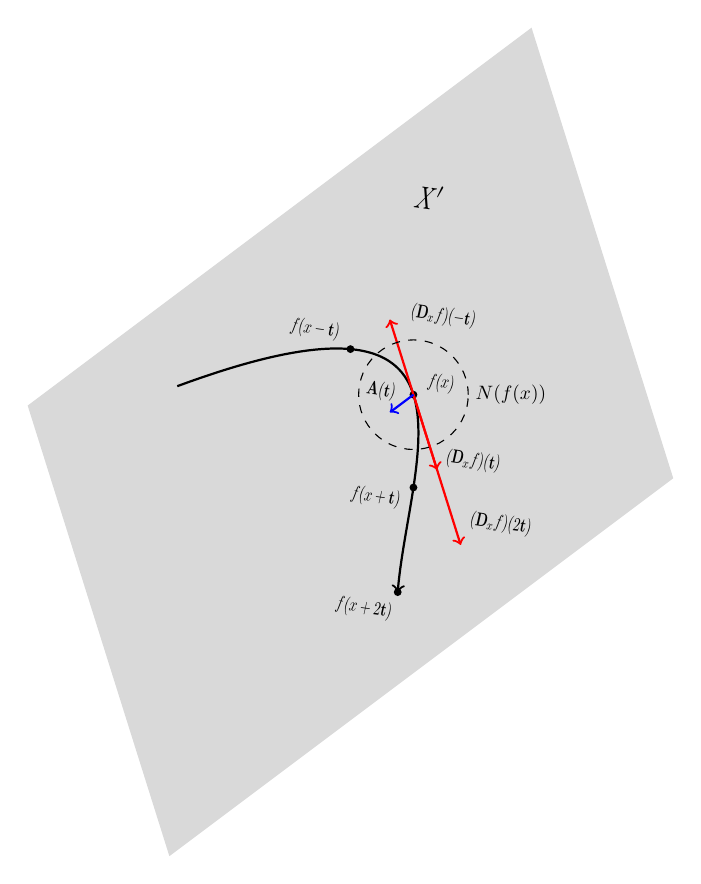
\begin{tikzpicture}[
    ->,
    plane x={(0.3,-0.9539)},
    plane y={(0.8,0.6)},
    canvas is plane,
]
    \fill[gray,fill opacity=0.3] (-3,-4) rectangle (3,4);
    \node at (-2,2) [rotate=52,transform shape] {$X'$};
    \node[circle,fill,inner sep=1pt] at (0,1) {};
 	\node at (0.1,1.4) [rotate=52,scale=0.6,transform shape] {$f(x)$};
    \node[circle,fill,inner sep=1pt] at (1,{5/8}) {};
 	\node at (0.8,0.1) [rotate=52,scale=0.6,transform shape] {$f(x+\mathbf{t})$};
    \node[circle,fill,inner sep=1pt] at (2,0) {};
 	\node at (1.9,-0.5) [rotate=52,scale=0.6,transform shape] {$f(x+2\mathbf{t})$};
    \node[circle,fill,inner sep=1pt] at (-1,{3/8}) {};
 	\node at (-1.5,0) [rotate=52,scale=0.6,transform shape] {$f(x-\mathbf{t})$};
	\draw[thick] plot[variable=\x,domain=-2:2,samples=73,smooth] 
 (\x,{1-\x*\x/2+\x*\x*\x/8});
 	\draw[thick,red] (0,1) -> (-1,1);
 	\node at (-0.6,1.7) [rotate=52,scale=0.6,transform shape] {$(\mathbf{D}_xf)(-\mathbf{t})$};
 	\draw[thick,red] (0,1) -> (1,1);
 	\node at (1.2,1.5) [rotate=52,scale=0.6,transform shape] {$(\mathbf{D}_xf)(\mathbf{t})$};
 	\draw[thick,red] (0,1) -> (2,1);
 	\node at (2.1,1.6) [rotate=52,scale=0.6,transform shape] {$(\mathbf{D}_xf)(2\mathbf{t})$};
 	\draw[thick,blue] (0,1) -> (0,{5/8});
 	\node at (-0.3,0.6) [rotate=52,scale=0.6,transform shape] {$\mathbf{A}(\mathbf{t})$};
    \node[label={[scale=0.7]0:$N(f(x))$},draw,dashed,circle,inner sep=14pt] at (0,1) {};
\end{tikzpicture}
\end{tabular}
\end{adjustbox}
\end{center}
\end{figure}

\begin{res} If $f$ has a derivative at $x$, it is unique.
\end{res}
\begin{proof} Let $\mathbf{d}$ and $\mathbf{d}'$ be distance functions in $X$ and $X'$, and $d$ and $d'$ be metrics in $X$ and $X'$. Suppose there are two derivatives $\mathbf{D}_x^1f$ and $\mathbf{D}_x^2f$, whose values differ for some $\mathbf{u}$ in $T_xX$. Suppose $d'((\mathbf{D}_x^1f)(\mathbf{u}),(\mathbf{D}_x^2f)(\mathbf{u}))=\delta>0$. Consider a neighborhood $N$ in $L(T_xX;T_{f(x)}X')$ of the zero linear map such that for all $\mathbf{A}\in N$, $d'(\mathbf{A}(\mathbf{u}),\mathbf{0}_{X'}) \le \delta/3$. By \hyperref[defderivat]{definition} of derivative, there is a neighborhood $N'$ of $x$ such that if $k\mathbf{u}\in N'$, then,
\begin{align*}
\mathbf{d}'\left( f(x),f(x+k\mathbf{u})\right) = \mathbf{d}'_{f(x)}\left( (\mathbf{D}_x^1f)(k\mathbf{u})+\mathbf{A}^1(k\mathbf{u})\right),\\
\mathbf{d}'\left( f(x),f(x+k\mathbf{u})\right) = \mathbf{d}'_{f(x)}\left( (\mathbf{D}_x^2f)(k\mathbf{u})+\mathbf{A}^2(k\mathbf{u})\right)
\end{align*}
for some $\mathbf{A}^1,\mathbf{A}^2\in N$. If follows
\[ \mathbf{d}'\left( (\mathbf{D}_x^1f)(k\mathbf{u}), (\mathbf{D}_x^2f)(k\mathbf{u}) \right) = \mathbf{d}'\left( \mathbf{A}^2(k\mathbf{u}), \mathbf{A}^1(k\mathbf{u})\right).\]
Then, by triangle inequality,
\begin{align*}
k\delta &= d'\left( (\mathbf{D}_x^1f)(k\mathbf{u}), (\mathbf{D}_x^2f)(k\mathbf{u}) \right) \\
&= d'\left( \mathbf{A}^2(k\mathbf{u}), \mathbf{A}^1(k\mathbf{u})\right) \\
&\le d'\left( \mathbf{A}^2(k\mathbf{u}), \mathbf{0}_{X'} \right) + d'\left( \mathbf{0}_{X'}, \mathbf{A}^1(k\mathbf{u}) \right) \le 2k\delta/3,
\end{align*}
a contradiction.
\end{proof}

\begin{res} If $X$ and $X'$ are \hyperref[defafsp]{affine spaces}, the derivative of $f:X\rightarrow X'$ at $x\in X$, if it exists, is given by
\[ (\mathbf{D}_xf)(\mathbf{t}) = \lim_{h \to 0} {\mathbf{d}'}_{f(x)}^{\leftarrow} \left( \frac{\mathbf{d}'\left( f(x),f(x+h\mathbf{t}) \right)}{h} \right)\]
where $\mathbf{d}'$ is the \hyperref[defafsp]{distance function} in $X'$.
\end{res}
\begin{cmnt*}
Proof omitted. The expression gives the value of the derivative for vector $\mathbf{t}$ in the tangent space $T_xX$. The derivative specifies a value for each $\mathbf{t}$. Note that scaling $t$ scales the derivative by the same factor. The job of ${\mathbf{d}'}_{f(x)}^{\leftarrow}$ is to convert a free vector to a bound vector.
\end{cmnt*}

\begin{defn}[Differentiability on Affine Spaces]\label{defdfrbla}
If $X$ and $X'$ are \hyperref[defafsp]{affine spaces}, a map $f:X\rightarrow X'$ is differentiable at $x\in X$ if $f$ has a derivative at $x$. It is differentiable\index{differentiable map on affine space} if it is differentiable at $x$ for all $x \in X$.
\end{defn}

\begin{defn}[Derivative on Affine Space]\label{defaderiv}
If $(X,T)$ and $(X',T')$ are \hyperref[defafsp]{affine spaces} with distance functions $\mathbf{d}$ and $\mathbf{d}'$, respectively, and $f:X\rightarrow X'$ is \hyperref[defdfrbla]{differentiable}, the derivative of $f$\index{derivative on affine space} is the map\index{$\hat{\mathbf{D}}f$}
\[ \hat{\mathbf{D}}f:X\rightarrow L(T;T'):x\mapsto \mathbf{d}_{f(x)}'(\mathbf{D}_x f) \mathbf{d}_x^{\leftarrow}.\]
\end{defn}

\begin{cmnt*}
The derivative at a point is defined as an operator that takes tangent vectors in one tangent space to tangent vectors in another tangent space. The derivative of the map (not just at a point) is defined to take a point (for example, $x$) in the affine space to the derivative at that point ($(\hat{\mathbf{D}}f)(x)=\mathbf{d}_{f(x)}'(\mathbf{D}_x f) \mathbf{d}_x^{\leftarrow}$), modified such that it takes free vectors (not bound) (for example, $t\in T_xX$) to free vectors (not bound) ($(\mathbf{d}_{f(x)}'(\mathbf{D}_x f) \mathbf{d}_x^{\leftarrow})(\mathbf{t})\in T_{f(x)}Y$). This enables us to consider the value of the derivative at different points applied to the same free vector.
\end{cmnt*}

\begin{defn}[Higher Order Derivative]\label{defhoderiv}
If $(X,T)$ and $(X',T')$ are \hyperref[defafsp]{affine spaces}, $(\hat{\mathbf{D}}^kf):X\rightarrow L^k(T;T')=\hat{\mathbf{D}}(\hat{\mathbf{D}}^{k-1}f)$\index{$\hat{\mathbf{D}}^kf$} for $k>1$ with $\hat{\mathbf{D}}^1f=\hat{\mathbf{D}}f$.
\end{defn}

\begin{cmnt*} From \autoref{resmptensr}, $(\hat{\mathbf{D}}^kf):X\rightarrow \underbrace{T^* \otimes T^* \otimes \cdots \otimes T^*}_{k \text{ times}} \otimes T'$.
\end{cmnt*}

\begin{defn}[Partial Derivative]\label{defpderiv}
Given \hyperref[defafsp]{affine spaces} $(X,T)$ and $(X',T')$ with basis $(\mathbf{b}_1,\cdots,\mathbf{b}_n)$ for $T$ and basis $(\mathbf{e}_1,\cdots,\mathbf{e}_m)$ for $T'$, a partial derivative\index{partial derivative} of 
$f:X\rightarrow X'$ is\index{$\partial_jf^i$}
\[ (\partial_jf^i):X\rightarrow \mathbb{R}:x\mapsto \lim_{h\to 0} \frac{\mathbf{e}^{i}(f(x+h\mathbf{b}_j))-\mathbf{e}^{i}(f(x))}{h}\]
where $(\mathbf{e}^1,\cdots,\mathbf{e}^m)$ is the \hyperref[defdbas]{dual basis} for dual space $T'^*$.
\end{defn}

\begin{cmnt*} A partial derivative is defined with respect to ``directions'' in both domain affine space and range affine space, once we define these directions. That requires specifying bases in each space. The value of a partial derivative is real as the components $\mathbf{e}^{i}$ are real.
\end{cmnt*}

\subsection{Manifolds}
\begin{defn}[Manifold]\label{defmfold}
A $C^k$ manifold\index{manifold} modeled on an \hyperref[defafsp]{affine space} $X$ is a \hyperref[defhtop]{Hausdorff topological space} $M$\index{$M$} together with a collection of \hyperref[defoset]{open sets} $\{U_a|a\in A\}$ in $M$ and corresponding maps $\phi_a:U_a\rightarrow X$, such that
\begin{enumerate}
\item $\cup_{a\in A}U_a=M$,
\item For each $a\in A$, $\phi_a$ defines a homeomorphism $U_a\rightarrow \phi_a(U_a)$, and
\item if $a,b\in A$ and $U_a \cap U_b \neq \emptyset$, then the composite $\phi_b \circ \phi_a^{\leftarrow}$ on the set $\phi_a(U_b)$ on which it is defined, is $C^k$.
\end{enumerate}
The pairs $(U_a,\phi_a)$ are called charts\index{chart} on $M$, and the set $\{(U_a,\phi_a)|a\in A\}$ is called an atlas\index{atlas}.
\end{defn}

\begin{cmnt*} In the third condition in the definition above, why shouldn't the composite map $\phi_b \circ \phi_a^{\leftarrow}$ be defined on the set $\phi_a(U_a \cap U_b)$ rather than $\phi_a(U_b)$?
\end{cmnt*}

\begin{defn}[Smooth Manifold]\label{defsmfold}
A smooth manifold\index{smooth manifold} is a $C^{\infty}$ manifold.
\end{defn}

\begin{defn}[Dimension of Manifold]\label{defdmfold}
The dimension dim($M$) of a manifold\index{dimension of manifold} $M$ is the dimension of the affine space it is modeled on. An $n$-manifold\index{$n$-manifold} is a manifold with dimension $n$.
\end{defn}

\begin{exmp}\label{exmpS2}
Consider unit 2-sphere, as in Exercise VII.2.1 of \citet{Dodson/Poston:1991}, defined as $S^2=\{(x^1,x^2,x^3)\in\mathbb{R}^3|(x^1)^2+(x^2)^2+(x^3)^2=1\}$\index{$S^2$}. It is a 2-dimensional manifold embedded in $\mathbb{R}^3$ with charts $(U_{1+},\phi_{1+})$, $(U_{1-},\phi_{1-})$, $(U_{1+},\phi_{1+})$, $(U_{1-},\phi_{1-})$, $(U_{1+},\phi_{1+})$, and $(U_{1-},\phi_{1-})$ defined with ``flattening maps'' as
\begin{align*}
U_{i+}&=\{(x^1,x^2,x^3)\in S^2|x^i>0\}, \,i=1,2,3, \\
U_{i-}&=\{(x^1,x^2,x^3)\in S^2|x^i<0\}, \,i=1,2,3 \\
\phi_{1s}&:U_{1s}\rightarrow \mathbb{R}^2:(x^1,x^2,x^3)\mapsto (x^2,x^3), \, s\in\{+,-\},\\
\phi_{2s}&:U_{2s}\rightarrow \mathbb{R}^2:(x^1,x^2,x^3)\mapsto (x^1,x^3), \, s\in\{+,-\}, \text{ and}\\
\phi_{3s}&:U_{3s}\rightarrow \mathbb{R}^2:(x^1,x^2,x^3)\mapsto (x^1,x^2), \, s\in\{+,-\}.
\end{align*}
The following figure shows the images of a circle in $S^2$ mapped to $\mathbb{R}^2$ using charts $(U_{1+},\phi_{1+})$, $(U_{2+},\phi_{2+})$, and $(U_{3+},\phi_{3+})$. Even though all charts map to the same $\mathbb{R}^2$, the figure shows them on three different planes for clarity. One of these images can be mapped to another through composite maps mentioned in \autoref{defmfold} of a manifold. For example,
\[ \phi_{2+}\circ\phi_{1+}^{\leftarrow}:\mathbb{R}^2\rightarrow\mathbb{R}^2:(x^2,x^3)\mapsto(\sqrt{1-(x^2)^2-(x^3)^2},x^3).\]
\begin{figure}[H]
\begin{center}
\begin{asy}
import solids;
import three;
settings.render=0;
settings.prc=false;
currentprojection=perspective(1,0.2,0.4);
size(10cm);
// distances: radius and length
real r=.4, ar=.5;
// sphere
revolution S=sphere(O,r);
draw(surface(S),green+white+opacity(0.5));
// axes
draw((0,0,0)--(0,ar,0),linewidth(0.5pt),Arrow3);
draw((0,0,0)--(0,0,ar),linewidth(0.5pt),Arrow3);
draw((0,0,0)--(ar,0,0),linewidth(0.5pt),Arrow3);
//circle on sphere using four arcs
real theta=pi/3, phi=pi/6, alpha = pi/18;
real x0=r*sin(theta)*cos(phi), y0=r*sin(theta)*sin(phi), z0=r*cos(theta);
real x1=r*sin(theta)*cos(phi-alpha/sin(theta)), y1=r*sin(theta)*sin(phi-alpha/sin(theta)), z1=r*cos(theta);
real x2=r*sin(theta+alpha)*cos(phi), y2=r*sin(theta+alpha)*sin(phi), z2=r*cos(theta+alpha);
real x3=r*sin(theta)*cos(phi+alpha/sin(theta)), y3=r*sin(theta)*sin(phi+alpha/sin(theta)), z3=r*cos(theta);
real x4=r*sin(theta-alpha)*cos(phi), y4=r*sin(theta-alpha)*sin(phi), z4=r*cos(theta-alpha);
draw(arc((x0,y0,z0),(x1,y1,z1),(x2,y2,z2)),yellow+linewidth(1pt));
draw(arc((x0,y0,z0),(x2,y2,z2),(x3,y3,z3)),yellow+linewidth(1pt));
draw(arc((x0,y0,z0),(x3,y3,z3),(x4,y4,z4)),yellow+linewidth(1pt));
draw(arc((x0,y0,z0),(x4,y4,z4),(x1,y1,z1)),yellow+linewidth(1pt));

//points on the path of circle (not drawn)
real x(real t) {return r*sin(theta+alpha*sin(t))*cos(phi+alpha*cos(t)/sin(theta+alpha*sin(t)));}
real y(real t) {return r*sin(theta+alpha*sin(t))*sin(phi+alpha*cos(t)/sin(theta+alpha*sin(t)));}
real z(real t) {return r*cos(theta+alpha*sin(t));}

//x-y projection
real x(real t) {return r*sin(theta+alpha*sin(t))*cos(phi+alpha*cos(t)/sin(theta+alpha*sin(t)));}
real y(real t) {return r*sin(theta+alpha*sin(t))*sin(phi+alpha*cos(t)/sin(theta+alpha*sin(t)));}
real z(real t) {return 0;}
path3 p=graph(x,y,z,0,2*pi,operator ..);
draw(p,yellow+dashed+linewidth(1));

//y-z projection
real x(real t) {return 0;}
real y(real t) {return r*sin(theta+alpha*sin(t))*sin(phi+alpha*cos(t)/sin(theta+alpha*sin(t)));}
real z(real t) {return r*cos(theta+alpha*sin(t));}
path3 p=graph(x,y,z,0,2*pi,operator ..);
draw(p,yellow+dashed+linewidth(1));

//z-x projection
real x(real t) {return r*sin(theta+alpha*sin(t))*cos(phi+alpha*cos(t)/sin(theta+alpha*sin(t)));}
real y(real t) {return 0;}
real z(real t) {return r*cos(theta+alpha*sin(t));}
path3 p=graph(x,y,z,0,2*pi,operator ..);
draw(p,yellow+dashed+linewidth(1));
\end{asy}
\end{center}
\end{figure}
\end{exmp}

\begin{defn}[Differentiability on Manifolds]\label{defdfrblm}
A map $f:M\rightarrow N$ between smooth manifolds is differentiable\index{differentiable map on manifold} at $x\in M$ if for some charts $(U,\phi)$ on $M$, $(V,\psi)$ on $N$, with $x\in U$, $f(x)\in V$, the map $\psi \circ f \circ \phi^{\leftarrow}$ is \hyperref[defdfrbla]{differentiable} at $\phi(x)$. The map $f$ is $C^k$ at $x$ if the map $\psi \circ f \circ \phi^{\leftarrow}$ is $C^k$ at $\phi(x)$. The map is differentiable if it is differentiable at all $x\in M$. The map is $C^k$ if it is $C^k$ at all $x\in M$.
\end{defn}

\begin{cmnt*}
Basically, the differentiability of a map on manifolds is defined in terms of differentiability of the corresponding map between their underlying affine spaces.
\end{cmnt*}

\begin{defn}[Diffeomorphism on Manifolds]\label{defdifm}
A homoemorphism $f:M\rightarrow N$ between $C^k$ manifolds is a $C^k$ diffeomorphism\index{diffeomorphism on manifolds} if both $f$ and $f^{\leftarrow}$ are $C^k$. Two manifolds are diffeomorphic\index{diffeomorphic} if there is a diffeomorphism between them.
\end{defn}

\begin{res} \label{resTuM}Let $M$ be a smooth manifold  modeled on an affine space $(X,T)$ with $u\in M$. Let  $(U,\phi)$, $(U',\phi')$ be charts on $M$ with $u\in U\cap U'$, and $\mathbf{t},\mathbf{t}'\in T$. Define relation $\sim$ by
\[ (U,\phi,\mathbf{t}) \sim (U',\phi',\mathbf{t}') \iff \left(\left(\hat{\mathbf{D}}\left(\phi' \circ \phi^{\leftarrow}\right)\right)\left(\phi(u)\right)\right)(\mathbf{t}) = \mathbf{t}'. \]
Then,
\begin{enumerate}
\item $\sim$ is an equivalence relation.
\item If $(U,\phi,\mathbf{t}) \sim (U',\phi',\mathbf{t}')$ and $(U,\phi,\mathbf{s}) \sim (U',\phi',\mathbf{s}')$, then
\[ (U,\phi,\mathbf{t}+\mathbf{s}) \sim (U',\phi',\mathbf{t}'+\mathbf{s}') \]
and
\[ (U,\phi,\mathbf{t}a) \sim (U',\phi',\mathbf{t}'a) \text{ for all } a\in\mathbb{R}.\]
\end{enumerate}
Hence, the set of $\sim$ equivalence classes is a vector space.
\end{res}
\begin{cmnt*}
Proof omitted. Two pairs of charts (around $u$) and tangent vectors in $T$ belong to the same equivalence class if the derivative of the composite map $\phi' \circ \phi^{\leftarrow}$ from the image under the first chart to the image under the second chart maps the first tangent vector to the second tangent vector. The composite map here is between affine spaces and hence its derivative is \hyperref[defderivat]{defined} already. \end{cmnt*}

\begin{cmnt*}
We used slightly different notation from \citet{Dodson/Poston:1991}. In the definition of the equivalence relation $\sim$, they specify the right side as $\hat{\mathbf{D}}_{\phi(u)}(\phi' \circ \phi^{\leftarrow})\mathbf{t} = \mathbf{t}'$ but the notation $\hat{\mathbf{D}}_{\phi(u)}$ has not been defined. We instead use
$((\hat{\mathbf{D}}(\phi' \circ \phi^{\leftarrow}))(\phi(u)))(\mathbf{t})$. Here, $\hat{\mathbf{D}}(\phi' \circ \phi^{\leftarrow})$ is the derivative of the composite map $\phi' \circ \phi^{\leftarrow}$. It is a map from points in $X$ to maps from free vectors in $T$ to free vectors in $T$. Its value at the point $\phi(u)$ is $(\hat{\mathbf{D}}(\phi' \circ \phi^{\leftarrow}))(\phi(u))$, a map from free vectors in $T$ to free vectors in $T$. Finally, its value at free vector $\mathbf{t}$ is $((\hat{\mathbf{D}}(\phi' \circ \phi^{\leftarrow}))(\phi(u)))(\mathbf{t})$, a free vector in $T$. The notation could have been simplified to $(\mathbf{D}_{\phi(u)}(\phi' \circ \phi^{\leftarrow}))(\mathbf{t}) = \mathbf{t}'$ if $\mathbf{t}$ and $\mathbf{t}'$ were bound vectors, but they need to be free vectors in this definition.
\end{cmnt*}

\begin{defn}[Tangent Space to a Manifold]\label{defTuM}
The tangent space\index{Tangent Space to a Manifold} $T_uM$\index{$T_uM$} to $M$ at $u$ is the vector space consisting of the set of $\sim$ equivalence classes defined in \autoref{resTuM}. Each equivalence class is a tangent vector to $M$ at $u$.
\end{defn}

\begin{cmnt*}
A tangent vector to a manifold is a vector in the complicated vector space of equivalence classes defined in \autoref{resTuM}. It can be represented as a vector in the affine space underlying the manifold once we pin down a chart $(U,\phi)$. The vector will be different if we choose a different chart. However, all those vector representations will be related by an equivalence class defined in \autoref{resTuM}.
\end{cmnt*}

\begin{res} \label{resTuM2}Let $M$ be a smooth manifold  modeled on an affine space $(X,T)$ and embedded in $\mathbb{R}^n$ with inclusion $\iota:M\rightarrow \mathbb{R}^n$. Let  $(U,\phi)$, $(U',\phi')$ be charts on $M$ with $u\in U\cap U'$, and $\mathbf{t},\mathbf{t}'\in T$, and $\sim$ be as defined in \autoref{resTuM}. Then
\[ (U,\phi,\mathbf{t}) \sim (U',\phi',\mathbf{t}') \iff \left(\left(\hat{\mathbf{D}}\left(\iota \circ \phi^{\leftarrow}\right)\right)\left(\phi(u)\right)\right)(\mathbf{t}) = \left(\left(\hat{\mathbf{D}}\left(\iota \circ \phi^{\leftarrow}\right)\right)\left(\phi'(u)\right)\right)(\mathbf{t}'). \]
Thus, each tangent vector to $M$ at $u$ is uniquely represented by a single vector  $\mathbf{s}\in T_{\iota(u)}\mathbb{R}^n$ such that for any $(U,\phi,\mathbf{t})$ in the equivalence class of that tangent vector, the derivative of the composite map $\iota \circ \phi^{\leftarrow}$ from the image under the chart $\phi$ to $\mathbb{R}^n$ maps $\mathbf{t}$ to $\mathbf{s}$.
\end{res}

\begin{cmnt*}
Proof omitted but probably follows from \autoref{resTuM} and Inverse Function Theorem as hinted in Exercise VII.2.5. The notation to the right of the equivalence operator has been changed and $T_u\mathbb{R}^n$ has been changed to $T_{\iota(u)}\mathbb{R}^n$ to be consistent with the rest of the notation.
\end{cmnt*}

\begin{res} \label{resEmbed}An $m$-dimensional manifold $M$ can be mapped smoothly and injectively into $\mathbb{R}^n$ for $n\ge N$ where $N\le 2m+1$. The map $\iota:M\rightarrow\mathbb{R}^n$ is called inclusion\index{inclusion}.
\end{res}

\begin{cmnt*}
Proof is supposed to be nontrivial. If $M\subset \mathbb{R}^n$, we indicate inclusion as $\iota:M\xhookrightarrow{}\mathbb{R}^n$\index{$\xhookrightarrow{}$} to emphasize that the domain of the inclusion is a subset of its range.
\end{cmnt*}

\begin{defn}[Derivative on Manifold]\label{defmderiv}
Let $M$ be a manifold  modeled on an affine space $(X,T)$ and $N$ be a manifold  modeled on an affine space $(Y,S)$. If $f:M\rightarrow N$ is differentiable at $u$ with chart $(U,\phi)$ on $M$, chart $(V,\psi)$ on $N$, $u\in U$, and $f(u)\in V$, then the derivative of $f$ at $u$\index{derivative on manifold} maps equivalence classes in $T_uM$ to $T_{f(u)}N$:
\begin{align*}
\mathbf{D}_uf:&T_uM\rightarrow T_{f(u)}N:\\
&[(U,\phi,\mathbf{t})]\mapsto [\left(V,\psi,\mathbf{D}_{\phi(u)}\left(\phi\circ f \circ \phi^{\leftarrow}\right)\mathbf{t}\right)]
\end{align*}\index{$\mathbf{D}_uf$}
where $\mathbf{t}\in T$. Here, $(U',\phi',\mathbf{t}')\in[(U,\phi,\mathbf{t})]$ iff $(U',\phi')$ is a chart on $M$ with $u\in U'$, $\mathbf{t}'\in T$,  and
\[ \left(\left(\hat{\mathbf{D}}\left(\phi' \circ \phi^{\leftarrow}\right)\right)\left(\phi(u)\right)\right)(\mathbf{t}) = \mathbf{t}'. \]
Similarly, $(V',\psi',\mathbf{s}')\in[(V,\psi,\mathbf{s})]$ iff $(V',\psi')$ is a chart on $M$ with $f(u)\in V'$, $\mathbf{s},\mathbf{s}'\in S$, and
\[ \left(\left(\hat{\mathbf{D}}\left(\psi' \circ \psi^{\leftarrow}\right)\right)\left(\psi(f(u))\right)\right)(\mathbf{s}) = \mathbf{s}'. \]
\end{defn}

\begin{cmnt*}
Exercise VII.I.6 in \citep{Dodson/Poston:1991} shows that $\mathbf{D}_uf$ is well-defined. That is, the definition does not depend on the specific choice of charts $(U,\phi)$ and $(V,\psi)$. Essentially, this requires one to show that if $(U,\phi)$ and $(U',\phi')$ are charts on $M$ with $u\in U\cap U'$, $(V,\psi)$ and $(V',\psi')$ are charts on $N$ with $f(u)\in V\cap V'$, $\mathbf{t},\mathbf{t}'\in T$, and $(U,\phi,\mathbf{t})\sim(U',\phi',\mathbf{t}')$, then,
\[ \left(V,\psi,\mathbf{D}_{\phi(u)}\left(\phi\circ f \circ \phi^{\leftarrow}\right)\mathbf{t}\right) \sim \left(V',\psi',\mathbf{D}_{\phi'(u)}\left(\phi'\circ f \circ \phi'^{\leftarrow}\right)\mathbf{t'}\right).\]
\end{cmnt*}

\begin{cmnt*}
If we fix one chart for $M$ and another for $N$, then the derivative $\mathbf{D}_uf$ maps a tangent vector in the affine space underlying $M$ (corresponding to a tangent vector in $M$, an equivalence class) to a tangent vector in the affine space underlying $N$ (corresponding to a tangent vector in $N$, an equivalence class). Picking specific charts (like picking basis or coordinate system) is innocuous as other chart choices will change vectors in affine spaces but they will still correspond to the same tangent vector equivalence classes in manifolds.
\end{cmnt*}

\subsection{Bundles and Fields}
\begin{res} \label{resTM}Suppose $M$ is an $n$-manifold  modeled on an affine space $X$ with atlas $\{(U_a,\phi_a)|a\in A\}$. Let $TM=\cup_{u\in M}T_uM$\index{$TM$} and  $TU_a=\cup_{u\in U_a}T_uM \subseteq TM$. Then, $\{(TU_a,\mathbf{D}\phi_a)|a\in A\}$ is an atlas making $TM$ a 2$n$-manifold modeled on $X\times X$, where $\mathbf{D}\phi_a:TU_a\rightarrow TX$ is defined by $\mathbf{D}\phi_a|_{T_uM}=\mathbf{D}_u\phi_a$\index{$\mathbf{D}\phi_a$}.
\end{res}

\begin{cmnt*}
For each $a\in A$, the atlas $\{(TU_a,\mathbf{D}\phi_a)\}$ takes a bound tangent vector on manifold from the set $TU_a$ to a bound tangent vector in $X\times X$ (specifying the starting and the ending points of the vector). Since $X$ is an affine space of dimension $n$, $X\times X$ is an affine space of dimension $2n$, so $TM$ is a 2$n$-manifold. The map $\mathbf{D}\phi_a$ is defined to be between manifolds and is constructed by using maps $\mathbf{D}_x\phi_a$ between vector spaces at each point $x$. The derivative of a map from one affine space to another was defined in \autoref{defaderiv} and the derivative of a map from one manifold to another was defined in \autoref{defmderiv}. $\mathbf{D}_u\phi_a$ is the derivative of a map $\phi_a$ from a manifold to an affine space, which is a trivial manifold.
\end{cmnt*}

\begin{proof} $TM$ is a manifold if it satisfies the three conditions in \autoref{defmfold}. First, the domains $TU_a$ of all charts cover $TM$. This follows from $TM=\cup_{u\in M}T_uM$.

\noindent Second, each chart $\mathbf{D}\phi_a$ defines a \hyperref[defhomeo]{homeomorphism}. Assign a topology to $TM$ with open sets consisting of finite intersections and arbitrary unions of sets of form $(\mathbf{D}\phi_a)^{\leftarrow}(W)$ where $a\in A$ and $W$ is an open set in $X \times X$. This ensures all $\mathbf{D}\phi_a$'s are continuous (see \autoref{rescontf}). $\mathbf{D}\phi_a$ defines a homeomorphism (\autoref{defhomeo}) because
\begin{enumerate}
\item $\mathbf{D}\phi_a$ is injective: Consider $\mathbf{t},\mathbf{t}'\in TU_a$ and $\mathbf{t}\neq \mathbf{t}'$.
\begin{enumerate}
\item  If $\mathbf{t}\in T_uM,u\in U_a,\mathbf{t}'\notin T_uM$, then $(\mathbf{D}\phi_a)(\mathbf{t}) \neq (\mathbf{D}\phi_a)(\mathbf{t}')$ because $(\mathbf{D}\phi_a)(\mathbf{t})\in T_{\phi_a(u)}X$ but $(\mathbf{D}\phi_a)(\mathbf{t}')\notin T_{\phi_a(u)}X$.
\item If $\mathbf{t},\mathbf{t}'\in T_uM,u\in U_a$, then $(\mathbf{D}\phi_a)(\mathbf{t}) \neq (\mathbf{D}\phi_a)(\mathbf{t}')$ because $\mathbf{D}\phi_a|_{T_uM}$, defined as $\mathbf{D}_u\phi_a$ is an isomorphism and hence injective. $\phi_a$ is a homeomorphism (see \autoref{defmfold}) but why is $\mathbf{D}_u\phi_a$ an isomorphism? From \autoref{defmderiv}, once a chart is fixed, $\mathbf{D}_u\phi_a$ is a linear map from tangent vectors in $X$ (corresponding to equivalence classes in $T_uM$) to tangent vectors in $X$. Fixing that chart to be $(U_a,\phi_a)$, $\mathbf{D}_u\phi_a$ is an identity map, and hence, an isomorphism.
\end{enumerate}
\item Similarly, $\mathbf{D}\phi_a$ is surjective because $\mathbf{D}_u\phi_a$ is an isomorphism.
\item $\mathbf{D}\phi_a$ is continuous (by the choice made above of the topology on $TM$).
\item $(\mathbf{D}\phi_a)^{\leftarrow}$ exists (because $\mathbf{D}\phi_a$ is injective) and is continuous (see \autoref{rescontf}) if for any open set $U$ in $TM$, $\left(\left(\mathbf{D}\phi_a\right)^{\leftarrow}\right)^{\leftarrow}(U)$ is open in $X\times X$. This holds if it holds for all $U$ of the form $(\mathbf{D}\phi_b)^{\leftarrow}(W)$ because 
open sets in $TM$ are finite intersections and arbitrary unions of sets of the form $(\mathbf{D}\phi_b)^{\leftarrow}(W)$. Thus, $(\mathbf{D}\phi_a)^{\leftarrow}$ is continuous if $\left(\left(\mathbf{D}\phi_a\right)^{\leftarrow}\right)^{\leftarrow}\left( (\mathbf{D}\phi_b)^{\leftarrow}(W) \right)$ is open in $X\times X$ for any open set $W$ in $X \times X$. But
\[ \left(\left(\mathbf{D}\phi_a\right)^{\leftarrow}\right)^{\leftarrow}\left( (\mathbf{D}\phi_b)^{\leftarrow}(W) \right) = \left(\mathbf{D}\phi_b \circ \left( \mathbf{D}\phi_a \right)^{\leftarrow} \right)^{\leftarrow}(W) \]
because if $\mathbf{y} \in \left(\left(\mathbf{D}\phi_a\right)^{\leftarrow}\right)^{\leftarrow}\left( (\mathbf{D}\phi_b)^{\leftarrow}(W) \right)$, then $\left(\mathbf{D}\phi_b \circ \left( \mathbf{D}\phi_a \right)^{\leftarrow} \right)(\mathbf{y})\in W$ and if $\mathbf{y} \in \left(\mathbf{D}\phi_b \circ \left( \mathbf{D}\phi_a \right)^{\leftarrow} \right)^{\leftarrow}(W)$, then $\left(\mathbf{D}\phi_a\right)^{\leftarrow}(\mathbf{y}) \in \left( (\mathbf{D}\phi_b)^{\leftarrow}(W) \right)$.
Thus, $(\mathbf{D}\phi_a)^{\leftarrow}$ is continuous if $\left(\mathbf{D}\phi_b \circ \left( \mathbf{D}\phi_a \right)^{\leftarrow} \right)^{\leftarrow}(W)$ is open in $X\times X$ for any open set $W$ in $X \times X$, or equivalently by \autoref{rescontf}, if $\mathbf{D}\phi_b \circ \left( \mathbf{D}\phi_a \right)^{\leftarrow}$ is continuous. But by chain rule, $\mathbf{D}\phi_b \circ \left( \mathbf{D}\phi_a \right)^{\leftarrow} = \mathbf{D}\left( \phi_b \circ \phi_a^{\leftarrow} \right)$, which is continuous because $\phi_b \circ \phi_a^{\leftarrow}$ is continuously differentiable by the \hyperref[defmfold]{definition} of charts in a manifold. 
\end{enumerate}

\noindent Third, for $a,b\in A$, the composite map $(\mathbf{D}\phi_b)(\mathbf{D}\phi_b)^{\leftarrow}$ is continuously differentiable (and similarly for higher order derivatives). The composite map takes bound tangent vectors in $X$ to bound tangent vectors in $X$. That is, points in $X \times X$ to $X \times X$. We now convert these bound vectors to a pairs of starting points and free vectors, thus converting the composite map to a map from points in $X \times T$ to points in $X \times T$. For this, we define a map converting a bound vector to a pair of starting point and a free vector:
\[ A:X \times X \rightarrow X \times T:(x,y)\mapsto \left(x,\mathbf{d}(x,y)\right)\]
where $\mathbf{d}$ is the \hyperref[defafsp]{distance function} in $X$. Now consider this modified composite map:
\begin{align*}
A\circ \left(\mathbf{D}\left(\phi_b\circ\phi_a^{\leftarrow}\right)\right)\circ A^{\leftarrow}:&\, \phi_a(U_a\cap U_b) \times T \rightarrow \phi_b(U_a\cap U_b) \times T \\
&(q,\mathbf{t})\mapsto \left( \left( \phi_b \circ \phi_a^{\leftarrow} \right) q, \hat{\mathbf{D}}\left( \phi_b \circ \phi_a^{\leftarrow} \right) \mathbf{t} \right) = (p,\mathbf{s}).
\end{align*}
The domain and range of this modified composite map are direct sum \citep[see][p. 180]{Dodson/Poston:1991}\index{direct sum} $X \oplus T$\index{$\oplus$} of affine space $X$ and tangent space $T$. The derivative of this map at $(q,\mathbf{t})$ is
\begin{align*}
\mathbf{D}_q\left( \phi_b \circ \phi_a^{\leftarrow} \right) \oplus \mathbf{D}_{\mathbf{t}}\left( \mathbf{D}_q\left( \phi_b \circ \phi_a^{\leftarrow}\right)\right): T_qX \oplus T_{\mathbf{t}}\left( T_qX\right) \rightarrow T_pX \oplus T_{\mathbf{s}}\left( T_pX\right).
\end{align*}
However, $\mathbf{D}_q\left( \phi_b \circ \phi_a^{\leftarrow}\right)$ is linear (all derivatives are) so its derivative is a constant and doesn't depend on $\mathbf{t}$. Thus, the derivative of the modified composite map can be ``identified with'' (is isomorphic to?) with
\begin{align*}
\mathbf{D}_q\left( \phi_b \circ \phi_a^{\leftarrow} \right) \oplus \mathbf{D}_q\left( \phi_b \circ \phi_a^{\leftarrow}\right): T_qX \oplus T_qX \rightarrow T_pX \oplus  T_pX.
\end{align*}
Now going back to the original composite map, by Chain Rule,
\begin{align*}
\mathbf{D}_{(q,\mathbf{t})}\left( (\mathbf{D}\phi_b) \circ \left( \mathbf{D}\phi_a \right)^{\leftarrow} \right) &= \mathbf{D}_{(q,\mathbf{t})}\left( \mathbf{D}(\phi_b\circ\phi_a^{\leftarrow} )\right) \\
&= \mathbf{D}_{(q,\mathbf{t})}\left( A^{\leftarrow} \circ \left( A \circ \mathbf{D}(\phi_b\circ\phi_a^{\leftarrow} ) \circ A^{\leftarrow} \right) \circ A \right) \\
&= \mathbf{A}^{\leftarrow} \circ \left( \mathbf{D}_q\left( \phi_b \circ \phi_a^{\leftarrow} \right) \oplus \mathbf{D}_q\left( \phi_b \circ \phi_a^{\leftarrow}\right) \right) \circ \mathbf{A}
\end{align*}
which exists and is continuous because $\phi_b\circ \phi_a^{\leftarrow}$ is continuously differentiable by the \hyperref[defmfold]{definition} of charts in a manifold.
\end{proof}

\begin{exmp}\label{exmpTM}
Consider the manifold $S^2$ with its associated charts in Example \ref{exmpS2}. It is embedded in $\mathbb{R}^3$ with inclusion $\iota:S^2\xhookrightarrow{}\mathbb{R}^n:(u^1,u^2,u^3)\mapsto(u^1,u^2,u^3)$. Consider $u=(u^1,u^2,u^3)\in S^2$ with $u^1,u^2,u^3>0$. Let us use the notation $\overrightarrow{(v^1,v^2,v^3)}$ to indicate the vector from $(0,0,0)$ to $(v^1,v^2,v^3)$. A vector $\mathbf{v}=\overrightarrow{(v^1,v^2,v^3)}$ with $v^1,v^2,v^3\in\mathbb{R}$ is tangent to $S^2$ at $u$ in $\mathbb{R}^3$ if $u^1v^1+u^2v^2+u^3v^3=0$. By \autoref{resTuM2}, each such $\mathbf{v}$ represents (an equivalence class corresponding to) a tangent vector in $T_uS^2$, a tangent to $S^2$ at $u$. Denote this by $[\mathbf{v}]$. Consider $(U_{1+},\phi_{1+},\mathbf{t}_{1+}) \in [\mathbf{v}]$. This requires $((\hat{\mathbf{D}}(\iota \circ \phi_{1+}^{\leftarrow}))(\phi_{1+}(u)))(\mathbf{t}_{1+})=\mathbf{v}$.
Since $\iota \circ \phi_{1+}^{\leftarrow}:\overrightarrow{(x^2,x^3)}\mapsto(\sqrt{1-(x^2)^2-(x^3)^2},x^2,x^3),$ we have
\begin{align*}
\tiny
&(\hat{\mathbf{D}}\iota \circ \phi_{1+}^{\leftarrow}((u^2,u^3)))(\overrightarrow{(w^2,w^3)}) \\
&= \lim_{h\to 0}\frac{1}{h}[ (\sqrt{1-(u^2+hw^2)^2-(u^3+hw^3)^2},u^2+hw^2,u^3+hw^3) \\
&-(\sqrt{1-(u^2)^2-(u^3)^2},u^2,u^3)]\\
&=(\frac{-u^2w^2-u^3w^3}{\sqrt{1-(u^2)^2-(u^3)^2}},w^2,w^3)=(\frac{-u^2w^2-u^3w^3}{u^1},w^2,w^3).
\end{align*}
Then, $(U_{1+},\phi_{1+},\mathbf{t}_{1+}) \in [\mathbf{v}]$ with $\mathbf{t}_{1+}=\overrightarrow{(w^2,w^3)}$ if $(\frac{-u^2w^2-u^3w^3}{u^1},w^2,w^3)=(v^1,v^2,v^3).$ This is true if $(w^2,w^3)=(v^2,v^3)$. Thus, $(U_{1+},\phi_{1+},\overrightarrow{(v^2,v^3)}) \in [\mathbf{v}]$. Similarly, $(U_{2+},\phi_{2+},\overrightarrow{(v^1,v^3)}) \in [\mathbf{v}]$ and $(U_{3+},\phi_{3+},\overrightarrow{(v^1,v^2)}) \in [\mathbf{v}]$. The following figure shows a red tangent vector to $S^2$ in $\mathbb{R}^3$ and its projections (in red) under $\phi_{1+}$, $\phi_{2+}$, and $\phi_{3+}$ on three planes as the members of the corresponding tangent vector equivalence class. The tangent space to $S^2$ at $u$ is the set of all such $[\mathbf{v}]$:
\[T_uS^2 = \left\{[\mathbf{v}]\middle|\mathbf{v}=\overrightarrow{\left(v^1,v^2,v^3\right)},v^1,v^2,v^3\in\mathbb{R},u^1v^1
+u^2v^2+u^3v^3=0\right\}.\]
The red and blue vectors in the following figure are part of the tangent space to $S^2$ at the same point.
Finally, aggregating $T_uS^2$ over all $u\in S^2$, we get
\begin{align*}
&TS^2=\cup_{u\in S^2}T_uS^2 =\\
&\biggl\{\left(\left(u^1,u^2,u^3\right),\left[\overrightarrow{\left(v^1,v^2,v^3\right)}\right]\right)\,\Big| \\
&u^1,u^2,u^3,v^1,v^2,v^3\in\mathbb{R},(u^1)^2+(u^2)^2+(u^3)^2=1,u^1v^1+u^2v^2+u^3v^3=0\biggr\}.
\end{align*}
The red, blue, pink, and orange vectors in the following figure are part of $TS^2$. $TS^2$ is a manifold with atlas $\{(TU_a,\mathbf{D}\phi_a)|a\in\{1+,1-,2+,2-,3+,3-\}\}$. One chart in this atlas is
\begin{align*}
&\mathbf{D}\phi_{1+}:TU_{1+}\rightarrow T\mathbb{R}^2:\left(\left(u^1,u^2,u^3\right),\overrightarrow{\left(v^1,v^2,v^3\right)}\right)\mapsto 
\left( \left(u^2,u^3\right),\overrightarrow{\left(v^2,v^3\right)}\right)
\end{align*}
where $(u^1)^2+(u^2)^2+(u^3)^2=1$ and $u^1v^1+u^2v^2+u^3v^3=0$.
To see that $TS^2$ is 4-dimensional, note that
\[ \{((u^1,u^2,u^3)| u^1,u^2,u^3\in\mathbb{R},(u^1)^2+(u^2)^2+(u^3)^2=1 \} \]
is 2-dimensional, and for a given $(u^1,u^2,u^3)$,
\[ \{ (v^1,v^2,v^3) )\,| v^1,v^2,v^3\in\mathbb{R}, u^1v^1+u^2v^2+u^3v^3=0\} \]
is also 2-dimensional.

\begin{figure}[H]
\begin{center}
\begin{asy}
import solids;
import three;
settings.render=0;
settings.prc=false;
currentprojection=perspective(1,0.2,0.4);
size(10cm);
// distances: radius and length
real r=.4, ar=.5;
// sphere
revolution S=sphere(O,r);
draw(surface(S),green+white+opacity(0.5));
// axes
draw((0,0,0)--(0,ar,0),linewidth(0.5pt),Arrow3);
draw((0,0,0)--(0,0,ar),linewidth(0.5pt),Arrow3);
draw((0,0,0)--(ar,0,0),linewidth(0.5pt),Arrow3);
//circle on sphere using four arcs
real theta=pi/3, phi=pi/6, alpha = pi/18;
real x0=r*sin(theta)*cos(phi), y0=r*sin(theta)*sin(phi), z0=r*cos(theta);
real x1=r*sin(theta)*cos(phi-alpha/sin(theta)), y1=r*sin(theta)*sin(phi-alpha/sin(theta)), z1=r*cos(theta);
real x2=r*sin(theta+alpha)*cos(phi), y2=r*sin(theta+alpha)*sin(phi), z2=r*cos(theta+alpha);
real x3=r*sin(theta)*cos(phi+alpha/sin(theta)), y3=r*sin(theta)*sin(phi+alpha/sin(theta)), z3=r*cos(theta);
real x4=r*sin(theta-alpha)*cos(phi), y4=r*sin(theta-alpha)*sin(phi), z4=r*cos(theta-alpha);
draw(arc((x0,y0,z0),(x1,y1,z1),(x2,y2,z2)),yellow+linewidth(1pt));
draw(arc((x0,y0,z0),(x2,y2,z2),(x3,y3,z3)),yellow+linewidth(1pt));
draw(arc((x0,y0,z0),(x3,y3,z3),(x4,y4,z4)),yellow+linewidth(1pt));
draw(arc((x0,y0,z0),(x4,y4,z4),(x1,y1,z1)),yellow+linewidth(1pt));

//points on the path of circle (not drawn)
real x(real t) {return r*sin(theta+alpha*sin(t))*cos(phi+alpha*cos(t)/sin(theta+alpha*sin(t)));}
real y(real t) {return r*sin(theta+alpha*sin(t))*sin(phi+alpha*cos(t)/sin(theta+alpha*sin(t)));}
real z(real t) {return r*cos(theta+alpha*sin(t));}

//x-y projection
real x(real t) {return r*sin(theta+alpha*sin(t))*cos(phi+alpha*cos(t)/sin(theta+alpha*sin(t)));}
real y(real t) {return r*sin(theta+alpha*sin(t))*sin(phi+alpha*cos(t)/sin(theta+alpha*sin(t)));}
real z(real t) {return 0;}
path3 p=graph(x,y,z,0,2*pi,operator ..);
draw(p,yellow+dashed+linewidth(1));

//y-z projection
real x(real t) {return 0;}
real y(real t) {return r*sin(theta+alpha*sin(t))*sin(phi+alpha*cos(t)/sin(theta+alpha*sin(t)));}
real z(real t) {return r*cos(theta+alpha*sin(t));}
path3 p=graph(x,y,z,0,2*pi,operator ..);
draw(p,yellow+dashed+linewidth(1));

//z-x projection
real x(real t) {return r*sin(theta+alpha*sin(t))*cos(phi+alpha*cos(t)/sin(theta+alpha*sin(t)));}
real y(real t) {return 0;}
real z(real t) {return r*cos(theta+alpha*sin(t));}
path3 p=graph(x,y,z,0,2*pi,operator ..);
draw(p,yellow+dashed+linewidth(1));

real x5=x1+0.2*y1, y5=y1-0.2*x1, z5=z1;
draw((x1,y1,z1)--(x5,y5,z5),red+linewidth(0.5pt),Arrow3);
draw((x1,y1,0)--(x5,y5,0),red+dashed+linewidth(0.5pt),Arrow3);
draw((x1,0,z1)--(x5,0,z5),red+dashed+linewidth(0.5pt),Arrow3);
draw((0,y1,z1)--(0,y5,z5),red+dashed+linewidth(0.5pt),Arrow3);

real x6=x1-0.2*z1, y6=y1, z6=z1+0.2*x1;
draw((x1,y1,z1)--(x6,y6,z6),blue+linewidth(0.5pt),Arrow3);
draw((x1,y1,0)--(x6,y6,0),blue+dashed+linewidth(0.5pt),Arrow3);
draw((x1,0,z1)--(x6,0,z6),blue+dashed+linewidth(0.5pt),Arrow3);
draw((0,y1,z1)--(0,y6,z6),blue+dashed+linewidth(0.5pt),Arrow3);

real x7=x2-0.2*y2, y7=y2+0.2*x2, z7=z2;
draw((x2,y2,z2)--(x7,y7,z7),orange+linewidth(0.5pt),Arrow3);
draw((x2,y2,0)--(x7,y7,0),orange+dashed+linewidth(0.5pt),Arrow3);
draw((x2,0,z2)--(x7,0,z7),orange+dashed+linewidth(0.5pt),Arrow3);
draw((0,y2,z2)--(0,y7,z7),orange+dashed+linewidth(0.5pt),Arrow3);

real x8=x2, y8=y2-0.2*z2, z8=z2+0.2*y2;
draw((x2,y2,z2)--(x8,y8,z8),pink+linewidth(0.5pt),Arrow3);
draw((x2,y2,0)--(x8,y8,0),pink+dashed+linewidth(0.5pt),Arrow3);
draw((x2,0,z2)--(x8,0,z8),pink+dashed+linewidth(0.5pt),Arrow3);
draw((0,y2,z2)--(0,y8,z8),pink+dashed+linewidth(0.5pt),Arrow3);

\end{asy}
\end{center}
\end{figure}
\end{exmp}

\clearpage
\printindex

\bibliography{refs}
\end{document}

